\chapter{Resultados}

Em vista da teoria vigente na literatura e pelo que foi exposto no ponto de vista metodológico, 
obtiveram-se resultados e a análises nos contextos de condição anecóica, duto sem escoamento, 
duto com escoamento de exaustão e duto com escoamento sugado.

Para todos os resultados foi utilizada uma fonte acústica de 
natureza estacionária no começo do duto 
assim como é apresentada na Seção \ref{sec:modelo_numerico}.

Para análises da condição anecóica, históricos temporais de pressão e 
velocidade de partícula nas fronteiras do modelo numérico foram 
obtidos e usados para calcular coeficientes de reflexão. 
Esse procedimento foi realizado em vários pontos da camada de 
absorção acústica para melhor verificação de sua integridade acústica.

No que diz respeito a análises no contexto de duto sem escoamento,
 os parâmetros $|R_{r}|$ e $l/a$ foram calculados a partir dos 
históricos temporais de pressão e velocidade de partícula na terminação.
 Foi realizado também análise de convergência de malha para a obteção 
 da melhor acurácia frente a limitações computacionais.

Com uma malha definida e resultados validados no contexto 
sem escoamento, foram realizadas validações e análises 
com escoamento de exaustão. 
Para tanto, os parâmetros $|R_{r}|$ e $l/a$ foram calculados
 a partir dos históricos temporais de pressão e velocidade 
 de partícula na terminação para regimes subsônicos ($M$ $\leq$ 0,2).
  Isso possibilitou análises de $|R_{r}|$ com relação ao número de 
  Strouhal e explorar criticamente a amplificação acústica originada a 
  partir de um fenômeno fluidodinâmico. 

Em vista das fenomenologias fluidodinâmica e acústica validadas
 e analisadas no contexto de escoamento de exaustão,
  foram realizadas validações e análises para 
  a situação de escoamento de sucção. 
  Para tal fim, os parâmetros $|R_{r}|$ e $l/a$ foram 
  calculados a partir dos históricos temporais de 
  pressão e velocidade de partícula na terminação para 
  regimes subsônicos ($M$ $\leq$ 0,2). 
  Por carência de estudos que abordam o fenômeno de 
  escoamento sugado, vale ressaltar que o coloário de 
  Howe foi utilizado para a investigação dos 
  comportamentos de $|R_{r}|$ frente a diferentes números de Mach.

\section{Análise da Condição Anecóica}

Com a finalidade de mensurar e analisar o comportamento da
 condição de contorno anecóica por meio de 
 métricas numéricas e objetivas, foram calculados 
 impedâncias e coeficientes de reflexão nas 
 fronteiras do modelo numérico, ou seja, 
 nos pontos \textbf{A}, \textbf{B}, \textbf{C} e \textbf{D} 
 como é mostrado na Figura \ref{fig:modelo}. 
 As Figuras \ref{fig:impedancia_anecoica} e \ref{fig:abs_r_anecoica}
 apresentam esses resultados respectivamente. 

% \begin{figure}
% \begin{center}
% \begin{tikzpicture}
% \begin{axis}[
%     title={},
%     width=0.9\textwidth,
%     height=0.45\textwidth,
%     xlabel={Frequência},
%     ylabel={Sensibilidade},
%     x unit={\space Hz \space},
% 	y unit={\space C/g \space},
%     ytick=data,
%     xmin=0,
%     ymin=0,
%     ymax=0.55,
%     legend pos=north west,
%     grid=minor, % Display a grid	
% 	grid style={dashed,gray!90}, % Set the style
% 	]
%      %\addplot[color=black,dashed,thick,mark=*,mark options={solid},smooth] table[x index=2,y index=3] {Data/Kollias_SBMR_095_exp.txt}; \label{Kollias_exp095}
%      %\addlegendentry{Experimental (Kollias)}
%       %\addplot[color=blue,semithick] table[x index=0,y index=1] {Data/Kollias_SBMR_095_exp.txt}; \label{Kollias_sim095}
%     %\addlegendentry{Simulação (Kollias)}
%              \addplot[color=black, thick] table[x index=0,y index=1] {dados/coeficiente_reflexao_anecoica/A_real.txt};
%              \addplot[color=black,dashed,  thick] table[x index=0,y index=1] {dados/coeficiente_reflexao_anecoica/A_imag.txt};
%               \label{Comsol_095}% \addlegendentry{Simulação (Comsol)}
% \end{axis}
% \end{tikzpicture}
%  \caption{Resposta em carga do acelerômetro para $r$ igual a 0,95.}
% \end{center}
% \end{figure}

\newcommand\scalexA{1}
\newcommand\scaleyA{1}
\newcommand\scalex{1}
\newcommand\scaley{1}
\newcommand\scaleA{0.5}

\begin{figure}[ht!]
\begin{subfigure}{\scaleA \textwidth}
  % parte real impedancia 
\begin{tikzpicture}
\begin{axis}[
width=\scalexA \textwidth,
height=\scaleyA \textwidth,
xmin=0,
xmax=2.5,
ymin=0,
ymax=1,
ytick distance=0.1,
xtick distance=0.5,
grid=major, % Display a grid  
%grid style={dashed,gray!90}, % Set the style
xlabel = \small{$ka$},
ylabel = \small{$\Re(Z)$},
 y tick label style={/pgf/number format/.cd,%
          scaled y ticks = false,
          set decimal separator={,},
          fixed},
      x tick label style={/pgf/number format/.cd,%
          scaled x ticks = false,
          set decimal separator={,},
          fixed}%
]

\addplot[color=black, mark=o, only marks] table[x index=0,y index=1] {dados/coeficiente_reflexao_anecoica/A_real.txt};
 \addplot[color=black, mark=square, only marks] table[x index=0,y index=1] {dados/coeficiente_reflexao_anecoica/B_real.txt};
 \addplot[color=black, mark=triangle, only marks] table[x index=0,y index=1] {dados/coeficiente_reflexao_anecoica/C_real.txt};
 \addplot[color=black, mark=x, only marks] table[x index=0,y index=1] {dados/coeficiente_reflexao_anecoica/D_real.txt};

\end{axis}
\end{tikzpicture}
\caption[Impedância $Z_{\textbf{A}}$]{}
\label{fig:parte_real}
%\caption[Impedância $Z_{\textbf{A}}$]{Resultado da impedância calculada no ponto $\textbf{A}$, próximo da condição anecóica localizada nas fronteiras do modelo numérico. A linha contínua representa a parte real e a linha tracejada representa a parte imaginária.}
\end{subfigure}%
\begin{subfigure}{\scaleA \textwidth}
  % parte imaginaria impedancia 
\begin{tikzpicture}
\begin{axis}[
width=\scalexA \textwidth,
height=\scaleyA \textwidth,
xmin=0,
xmax=2.5,
ymin=0,
ymax=0.55,
ytick distance=0.1,
xtick distance=0.5,
grid=major, % Display a grid  
%grid style={dashed,gray!90}, % Set the style
xlabel = \small{$ka$},
ylabel = \small{$\Im(Z)$},
 y tick label style={/pgf/number format/.cd,%
          scaled y ticks = false,
          set decimal separator={,},
          fixed},
      x tick label style={/pgf/number format/.cd,%
          scaled x ticks = false,
          set decimal separator={,},
          fixed}%
]

\addplot[color=black, mark=o, only marks] table[x index=0,y index=1] {dados/coeficiente_reflexao_anecoica/A_imag.txt};
 \addplot[color=black, mark=square, only marks] table[x index=0,y index=1] {dados/coeficiente_reflexao_anecoica/B_imag.txt};
 \addplot[color=black, mark=triangle, only marks] table[x index=0,y index=1] {dados/coeficiente_reflexao_anecoica/C_imag.txt};
 \addplot[color=black, mark=x, only marks] table[x index=0,y index=1] {dados/coeficiente_reflexao_anecoica/D_imag.txt};

\end{axis}
\end{tikzpicture}
\caption[Impedância $Z_{\textbf{A}}$]{}
\label{fig:parte_imaginaria}
%\caption[Impedância $Z_{\textbf{A}}$]{Resultado da impedância calculada no ponto $\textbf{A}$, próximo da condição anecóica localizada nas fronteiras do modelo numérico. A linha contínua representa a parte real e a linha tracejada representa a parte imaginária.}
\end{subfigure}
\caption[Resultados de impedância na condição anecóica]{Resultados da 
impedância $Z$ em termos de 
parte real (\ref{fig:parte_real}) e parte 
imaginária (\ref{fig:parte_imaginaria}) na condição
 anecóica localizada nas fronteiras do 
 modelo numérico. Os pontos com $\bigcirc$, $\square$, $\bigtriangleup$ e $\times$  
 apresentam os resultados para os pontos 
 \textbf{A}, \textbf{B}, \textbf{C} e \textbf{D} respectivamente.}
\label{fig:impedancia_anecoica}
\end{figure}

A Figura \ref{fig:impedancia_anecoica} apresenta os resultados da 
impedância $Z$ em termos de 
parte real (\ref{fig:parte_real}) e parte 
imaginária (\ref{fig:parte_imaginaria}) na condição
 anecóica localizada nas fronteiras do 
 modelo numérico. Pode-se observar pela Figura \ref{fig:parte_real} que a parte real da 
 impedância converge para o valor de $\rho_{0} c_{0}$ de referência na literatura para os pontos 
 \textbf{A}, \textbf{C} e \textbf{D},
  que em unidades do LBM possui o valor igual 0,57735. Porém, para o ponto \textbf{B}, 
  numa região de descontinuidade na direção $z$ e $y$, diverge consideravelmente de uma condição 
  anecóica ideal. Já a Figura \ref{fig:parte_imaginaria}, nos pontos \textbf{A}, \textbf{C} e \textbf{D},
  mostra que a parte imaginária da impedância possui valores próximos de 0, que é o ideal de uma situação 
  totalmente anecóica. Porém o ponto \textbf{B} diverge consideravelmente e possui valores mais altos na parte imaginária de $Z$.

\newpage
\begin{figure}[ht!]
\centering
  \begin{tikzpicture}
  \begin{axis}[
  width=0.8\textwidth,
  height=0.4\textwidth,
  % x tick label style={
  %     /pgf/number format/.cd,
  %         fixed,
  %         fixed zerofill,
  %         precision=1,
  %     /tikz/.cd
  % },
  xmin=0,
  xmax=2.4,
  ymin=0,
  ymax=1.4,
  ytick distance=0.2,
  xtick distance=0.5,
  grid=major, % Display a grid  
  %grid style={dashed,gray!90}, % Set the style
  xlabel = $ka$,
  ylabel = $|R|$,
   y tick label style={/pgf/number format/.cd,%
          scaled y ticks = false,
          set decimal separator={,},
          fixed},
      x tick label style={/pgf/number format/.cd,%
          scaled x ticks = false,
          set decimal separator={,},
          fixed}%
  ]
 \addplot[color=black, mark=o] table[x index=0,y index=1] {dados/coeficiente_reflexao_anecoica/A_abs.txt};
 \addplot[color=black, mark=square] table[x index=0,y index=1] {dados/coeficiente_reflexao_anecoica/B_abs.txt};
 \addplot[color=black, mark=triangle] table[x index=0,y index=1] {dados/coeficiente_reflexao_anecoica/C_abs.txt};
 \addplot[color=black, mark=x] table[x index=0,y index=1] {dados/coeficiente_reflexao_anecoica/D_abs.txt};

  \end{axis}
  \end{tikzpicture}
  \caption[Coeficiente de reflexão $|R|$ na condição anecóica.]{Resultados do coeficiente de reflexão $|R|$ na condição anecóica localizada nas fronteiras do 
 modelo numérico. Os pontos com $\bigcirc$, $\square$, $\bigtriangleup$ e $\times$  
 apresentam os resultados para os pontos 
 \textbf{A}, \textbf{B}, \textbf{C} e \textbf{D} respectivamente.}
  \label{fig:abs_r_anecoica}
\end{figure}


A Figura \ref{fig:abs_r_anecoica} apresenta os resultados do coeficiente de reflexão $|R|$ na condição anecóica localizada nas fronteiras do 
 modelo numérico. Pode-se observar que, para os pontos \textbf{A}, \textbf{C} e \textbf{D},
  o coeficiente de reflexão é abaixo de 20\% para $ka$ $>$ 0,4, 
  somente nas baixas frequências $ka$ $<$ 0,4 há uma divergência, que pode ser atribuída
   a escolha dos parâmetros da condição anecóica como por exemplo espessura e coeficiente de absorção.
   Já o ponto \textbf{B} diverge de uma condição anecóica ideal, pois $R$ possui o valor de média 40\% na média, 
   pode-se atribuir esse fato pela localização desse ponto numa região de descontinuidade da camada de absorção acústica.

Em vista do que foi exposto, a camada de absorção acústica localizada nas fronteiras do domínio numérico
 possui um comportamento anecóico considerável. Mesmo no ponto \textbf{B} possuir divergências, 
 essa camada possui um comportamento aproximadamente anecóico em todo o restante dos pontos.
 Vale ressaltar também que, segundo o estudo de \citeonline{allam2006investigation}, 
 mesmo com paredes totalmente rígidas e refletoras, a acústica interna não é influenciada pelas reflexões do ambiente quando a terminação está a uma distância maior ou igual a de aproximadamente $79,5a$ da parede, sendo $a$ o raio do duto.  

\newpage
\section{Duto sem Escoamento}

A primeira etapa de validação do modelo numérico abordado nesse trabalho consiste num duto sem escoamento e com fonte acústica variando nos valores de $0 \leq ka \leq 1,8$. Nessa etapa são calculados os coeficientes de reflexão e correção da terminação (ponto \textbf{P}) e comparados com os resultados de \citeonline{levine1948radiation}. Porém, considerando que para cada razão de elemento por comprimento de onda terá um custo computacional e acurácia nos resultados, é preciso realizar uma análise de convergência para mensurar qual discretização é mais adequada. Portanto foram avaliadas quatro tipos de discretização para representar o raio do duto: 20, 15, 10 e 5 células. Não foi possível realizar com raio maior que 20 devido a limitação de memória. A Figura \ref{fig:resultados_sem_escoamento} apresenta os resultados com as discretizações citadas.

\begin{figure}[h!]
\begin{subfigure}{\scaleA \textwidth}
  \begin{tikzpicture}
  \begin{axis}[
  width=\scalex \textwidth,
  height=\scaley \textwidth,
  xmin=0,
  xmax=1.8,
  ymin=0.3,
  ymax=1,
  ytick distance=0.1,
  grid=major, % Display a grid  
  %grid style={dashed,gray!90}, % Set the style
  xlabel = \small{$ka$},
  ylabel = \small{$|R_{r}|$},
   y tick label style={/pgf/number format/.cd,%
          scaled y ticks = false,
          set decimal separator={,},
          fixed},
      x tick label style={/pgf/number format/.cd,%
          scaled x ticks = false,
          set decimal separator={,},
          fixed}%
  ]
 \addplot[color=black, thick] table[x index=0,y index=1] {dados/duto_sem_escoamento/analytical_data_abs_r.txt};
 \addplot[color=black, mark=o, only marks] table[x index=0,y index=1] {dados/duto_sem_escoamento/simulation_data_abs_r.txt};
   
  \end{axis}
  \end{tikzpicture}
  \caption[Coeficiente de Reflexão $R_{r}$ sem Escoamento]{}
  \label{fig:abs_r_sem_escoamento}
\end{subfigure}%
\begin{subfigure}{\scaleA \textwidth}
  \begin{tikzpicture}
  \begin{axis}[
  width=\scalex \textwidth,
  height=\scaley \textwidth,
  xmin=0,
  xmax=1.8,
    ymin=0,
    ymax=0.8,
    ytick distance=0.1,
    grid=major, % Display a grid  
  %grid style={dashed,gray!90}, % Set the style
  xlabel = \small{$ka$},
  ylabel = \small{$l/a$},
   y tick label style={/pgf/number format/.cd,%
          scaled y ticks = false,
          set decimal separator={,},
          fixed},
      x tick label style={/pgf/number format/.cd,%
          scaled x ticks = false,
          set decimal separator={,},
          fixed}%
  ]
 \addplot[color=black, thick] table[x index=0,y index=1] {dados/duto_sem_escoamento/analytical_data_loa.txt};
 \addplot[color=black, mark=o, only marks] table[x index=0,y index=1] {dados/duto_sem_escoamento/simulation_data_loa.txt};
   
  \end{axis}
  \end{tikzpicture}
  \caption[Coeficiente de Correção da Terminação $l/a$ sem Escoamento]{}
  \label{fig:loa_sem_escoamento}
\end{subfigure}
\caption[Resultados de $|R_{r}|$ e $l/a$ sem escoamento]{Resultados de $|R_{r}|$ (\ref{fig:abs_r_sem_escoamento}) e $l/a$ (\ref{fig:loa_sem_escoamento}) para duto sem escoamento. As linhas contínuas representam os resultados do modelo analítico exato de \citeonline{levine1948radiation} e os pontos $\bigcirc$, $\bigtriangleup$, $\square$ e $\times$ apresentam os resultados para 20, 15, 10 e 5 elementos de discretização para representar o raio do duto respectivamente.}
\label{fig:resultados_sem_escoamento}
\end{figure}

É possível percebecer da Figura \ref{fig:resultados_sem_escoamento} que a medida que a discretização vai aumentando mais o modelo numérico converge para o valor da literatura do modelo analítico. É possível perceber que a melhor discretização é a de 20 elementos para descrever o tamanho do raio. Vale ressaltar que a tabela \ref{table:discretizacao} apresenta esse fato com vistas no tamanho do raio ($a$), número de elementos representativos ($\gamma$) para $ka = 1,8$ e as correlações $r_r$, obtidas da Equação \ref{eq:correlacao}, para coeficiente de reflexão e $r_l$ para correção da terminação.    

\begin{table}[ht!]
\centering
\caption{Tamanho do raio, números de elementos representativos para $ka = 1,8$ e correlações.}
\label{table:discretizacao}
    \begin{tabular}{|l|l|l|l|}
        \hline
        $a$ & $\gamma$ & $r_r$ & $r_l$ \\ \hline
        20  & 70 & 99,95 \%  & 96,23 \%  \\ \hline
        15  & 52 &  86,08 \% & 86,84 \% \\ \hline
        10  & 35 &  70,65 \% & 68,43 \% \\ \hline
        5   & 17 &  61,23 \% & 48,06 \%  \\
        \hline
    \end{tabular}
\end{table}

A partir de uma discretização de $a = 20$ os resultados numéricos passam a ser razoavelemente aderentes com os da literatura. A Figura \ref{fig:abs_r_sem_escoamento} apresenta um alto coeficiente de reflexão para baixas frequências e o mesmo vai decaindo a medida em que a frequência aumenta. A Figura \ref{fig:loa_sem_escoamento} reflete a mesma atuação da inércia sobre as ondas acústicas, resultando num alto coeficiente de correção da terminação para baixas frequências e a diminuição do mesmo a medida que a frequência aumenta.       

% Comentar as correlações abaixo
% correlation =

    %0.7226


%correlation =

    %0.7217


%correlation =

    %0.8608


%correlation =

    %0.8584


%correlation =

    %0.9053


%correlation =

    %0.8990

\newpage
\section{Duto com Escoamento Subsônico de Exaustão}

Visto que o modelo numérico abordado está validado num contexto sem escoamento com uma discretização de elementos significativa ($a = 20$), há a necessidade de validá-lo com escoamento de exaustão usando os resultados na literatura desenvolvidos por \citeonline{munt1990acoustic}. Para isso foram escolhidos os números de Mach 0,07, 0,10, 0,15 e 0,20 para atender o requisito de  análises com escoamento de exaustão para $M \leq 0,2$.

\begin{figure}[ht!]
\begin{subfigure}{\scaleA \textwidth}
  \begin{tikzpicture}
  \begin{axis}[
  width=\scalex \textwidth,
  height=\scaley \textwidth,
  xmin=0,
  xmax=1.8,
    ymin=0.4,
    ymax=1.2,
    ytick distance=0.1,
    grid=major, % Display a grid  
  %grid style={dashed,gray!90}, % Set the style
  xlabel = \small{Número de Helmholtz ($ka$)},
  ylabel = \small{Coeficiente de Reflexão ($R_{r}$)},
  ]
 \addplot[color=black, thick] table[x index=0,y index=1] {dados/duto_exaustao/abs_r_007_analytical.txt};
 \addplot[color=black, mark=o, only marks] table[x index=0,y index=1] {dados/duto_exaustao/abs_r_007_simulation.txt};
   
  \end{axis}
  \end{tikzpicture}
  \caption[Coeficiente de Reflexão $R_{r}$ com Escoamento de Exaustão (M $=$ 0,07)]{}
  \label{fig:abs_r_exaustao_007}
\end{subfigure}%
\begin{subfigure}{\scaleA \textwidth}
  \begin{tikzpicture}
  \begin{axis}[
   width=\scalex \textwidth,
  height=\scaley \textwidth,
  xmin=0,
  xmax=1.8,
    ymin=0,
    ymax=0.9,
    ytick distance=0.1,
    grid=major, % Display a grid  
  %grid style={dashed,gray!90}, % Set the style
  xlabel = \small{$ka$},
  ylabel = \small{$l/a$},
   y tick label style={/pgf/number format/.cd,%
          scaled y ticks = false,
          set decimal separator={,},
          fixed},
      x tick label style={/pgf/number format/.cd,%
          scaled x ticks = false,
          set decimal separator={,},
          fixed}%
  ]
 \addplot[color=black, thick] table[x index=0,y index=1] {dados/duto_exaustao/loa_007_analytical.txt};
 \addplot[color=black, mark=o, only marks] table[x index=0,y index=1] {dados/duto_exaustao/loa_007_simulation.txt};
   
  \end{axis}
  \end{tikzpicture}
  \caption[Coeficiente de Correção da Terminação $l/a$ com Escoamento de Exaustão (M $=$ 0,07)]{}
  \label{fig:loa_exaustao_007}
\end{subfigure}
\caption[Resultados de $|R_{r}|$ e $l/a$ com escoamento de exaustão ($M =$ 0,07 e $Re =$ 1930,23)]{Resultados de $|R_{r}|$ (\ref{fig:abs_r_exaustao_007}) e $l/a$ (\ref{fig:loa_exaustao_007}) com escoamento de exaustão ($M =$ 0,07 e $Re =$ 1930,23). As linhas contínuas representam os resultados do estudo de \citeonline{munt1990acoustic} e os pontos circulares representam os resultados do modelo numérico.}
\label{fig:resultados_exaustao_007}
\end{figure}

A Figura \ref{fig:resultados_exaustao_007} apresenta os resultados da magnitude do coeficiente de reflexão $|R_{r}|$ (\ref{fig:abs_r_exaustao_007}) e do coeficiente de correção da terminação $l/a$ (\ref{fig:loa_exaustao_007}), calculados no ponto $\textbf{P}$ na terminação do duto com escoamento de exaustão: número de Mach $M =$ 0,07 e número de Reynolds $Re =$ 1930,23.  As correlações entre os resultados foram de 99,83 \% para o coeficiente de reflexão $|R_{r}|$ (\ref{fig:abs_r_exaustao_007}) e 87,76 \% para o coeficiente de correção da terminação $l/a$ (\ref{fig:loa_exaustao_007}). Apesar da Figura \ref{fig:loa_exaustao_007} apresentar boa correlação com os resultados analíticos exatos do estudo de \citeonline{munt1990acoustic}, há uma divergência para baixas frequências que pode ser explicada pelo fato da parede do duto ter a espessura de 10\% do raio do duto, o contrário da parede com espessura nula do modelo. Tal fato é abordado nos trabalhos de \citeonline{ando1969sound}, \citeonline{peters1993} e \citeonline{english2010}, que apresentam mudanças significativas de $l/a$ tendo em vista espessuras maiores do que o modelo de \citeonline{munt1990acoustic}.

A Figura \ref{fig:resultados_exaustao_010} apresenta os resultados da magnitude do coeficiente de reflexão $|R_{r}|$ (\ref{fig:abs_r_exaustao_010}) e do coeficiente de correção da terminação $l/a$ (\ref{fig:loa_exaustao_010}), calculados no ponto $\textbf{P}$ na terminação do duto com escoamento de exaustão: número de Mach $M =$ 0,10 e número de Reynolds $Re =$ 2757,42.  As correlações entre os resultados foram de 99,85 \% para o coeficiente de reflexão $|R_{r}|$ (\ref{fig:abs_r_exaustao_010}) e 95,02 \% para o coeficiente de correção da terminação $l/a$ (\ref{fig:loa_exaustao_010}). Apesar da Figura \ref{fig:loa_exaustao_010} apresentar boa correlação com os resultados analíticos exatos do estudo de \citeonline{munt1990acoustic}, há uma divergência nas baixas frequências ocasinada pela mesma razão já comentada na Figura \ref{fig:resultados_exaustao_007}. Pode-se ressaltar ainda que o pico da Figura \ref{fig:abs_r_exaustao_010} é maior que o da Figura \ref{fig:abs_r_exaustao_007} e se localiza numa região de mais alta frequência.

\begin{figure}[ht!]
\begin{subfigure}{\scaleA \textwidth}
  \begin{tikzpicture}
  \begin{axis}[
 width=\scalex \textwidth,
  height=\scaley \textwidth,
  xmin=0,
  xmax=1.8,
    ymin=0.4,
    ymax=1.2,
    ytick distance=0.1,
    grid=major, % Display a grid  
  %grid style={dashed,gray!90}, % Set the style
  xlabel = \small{Número de Helmholtz ($ka$)},
  ylabel = \small{Coeficiente de Reflexão ($R_{r}$)},
  ]
 \addplot[color=black, thick] table[x index=0,y index=1] {dados/duto_exaustao/abs_r_010_analytical.txt};
 \addplot[color=black, mark=o, only marks] table[x index=0,y index=1] {dados/duto_exaustao/abs_r_010_simulation.txt};
   
  \end{axis}
  \end{tikzpicture}
  \caption[Coeficiente de Reflexão $R_{r}$ com Escoamento de Exaustão (M $=$ 0,10)]{}
  \label{fig:abs_r_exaustao_010}
\end{subfigure}%
\begin{subfigure}{\scaleA \textwidth}
  \begin{tikzpicture}
  \begin{axis}[
  width=\scalex \textwidth,
  height=\scaley \textwidth,
  xmin=0,
  xmax=1.8,
    ymin=0.15,
    ymax=0.6,
    ytick distance=0.05,
    grid=major, % Display a grid  
  %grid style={dashed,gray!90}, % Set the style
  xlabel = \small{$ka$},
  ylabel = \small{$l/a$},
  ]
 \addplot[color=black, thick] table[x index=0,y index=1] {dados/duto_exaustao/loa_010_analytical.txt};
 \addplot[color=black, mark=o, only marks] table[x index=0,y index=1] {dados/duto_exaustao/loa_010_simulation.txt};
   
  \end{axis}
  \end{tikzpicture}
  \caption[Coeficiente de Correção da Terminação $l/a$ com Escoamento de Exaustão (M $=$ 0,10)]{}
  \label{fig:loa_exaustao_010}
\end{subfigure}
\caption[Resultados de $|R_{r}|$ e $l/a$ com escoamento de exaustão ($M =$ 0,10 e $Re =$ 2757,42)]{Resultados de $|R_{r}|$ (\ref{fig:abs_r_exaustao_010}) e $l/a$ (\ref{fig:loa_exaustao_010}) com escoamento de exaustão ($M =$ 0,10 e $Re =$ 2757,42). As linhas contínuas representam os resultados do estudo de \citeonline{munt1990acoustic} e os pontos circulares representam os resultados do modelo numérico.}
\label{fig:resultados_exaustao_010}
\end{figure}

A Figura \ref{fig:resultados_exaustao_015} apresenta os resultados de $|R_{r}|$ (\ref{fig:abs_r_exaustao_015}) e  $l/a$ (\ref{fig:loa_exaustao_015}) nas mesmas condições das Figuras \ref{fig:resultados_exaustao_007} e \ref{fig:resultados_exaustao_010}, porém para o número de Mach $M =$ 0,15 e número de Reynolds $Re =$ 2057,71.  As correlações entre os resultados foram de 99,80 \% para o coeficiente de reflexão $|R_{r}|$ (\ref{fig:abs_r_exaustao_015}) e 94,28 \% para o coeficiente de correção da terminação $l/a$ (\ref{fig:loa_exaustao_015}). A Figura \ref{fig:loa_exaustao_015} apresenta as mesmas divergências ocorridas nas Figuras \ref{fig:loa_exaustao_007} e \ref{fig:loa_exaustao_010}, eclodidas pelas mesmas razões. Vale ressaltar que apesar do número de Mach dos resultados da Figura \ref{fig:resultados_exaustao_015} serem maiores do que dos resultados da Figura \ref{fig:resultados_exaustao_010}, o número de Reynolds é menor, ou seja, com objetivo de verificar a influência do número de Reynolds a viscosidade do fluido foi alterada, inserindo a frequência de colisão como 1,98. Nesse sentido, subtende-se que os coeficientes de reflexão e de correção da terminação são insensíveis ao número de Reynolds. Tal fato é ratificado pelo fato das correlações serem congruentes entre si: 99,85 \% e 99,80 \% para $|R_{r}|$ e 95,02 \% e 94,28 \% para $l/a$.

\begin{figure}[ht!]
\begin{subfigure}{\scaleA \textwidth}
  \begin{tikzpicture}
  \begin{axis}[
  width=\scalex \textwidth,
  height=\scaley \textwidth,
  xmin=0,
  xmax=1.8,
    ymin=0.4,
    ymax=1.2,
    ytick distance=0.1,
    grid=major, % Display a grid  
  %grid style={dashed,gray!90}, % Set the style
  xlabel = \small{$ka$},
  ylabel = \small{$|R_{r}|$},
  ]
 \addplot[color=black, thick] table[x index=0,y index=1] {dados/duto_exaustao/abs_r_015_analytical.txt};
 \addplot[color=black, mark=o, only marks] table[x index=0,y index=1] {dados/duto_exaustao/abs_r_015_simulation.txt};
   
  \end{axis}
  \end{tikzpicture}
  \caption[Coeficiente de Reflexão $R_{r}$ com Escoamento de Exaustão (M $=$ 0,15)]{}
  \label{fig:abs_r_exaustao_015}
\end{subfigure}%
\begin{subfigure}{\scaleA \textwidth}
  \begin{tikzpicture}
  \begin{axis}[
  width=\scalex \textwidth,
  height=\scaley \textwidth,
  xmin=0,
  xmax=1.8,
    ymin=0.15,
    ymax=0.55,
    ytick distance=0.05,
    grid=major, % Display a grid  
  %grid style={dashed,gray!90}, % Set the style
  xlabel = \small{Número de Helmholtz ($ka$)},
  ylabel = \small{Correção da Terminação ($l/a$)},
  ]
 \addplot[color=black, thick] table[x index=0,y index=1] {dados/duto_exaustao/loa_015_analytical.txt};
 \addplot[color=black, mark=o, only marks] table[x index=0,y index=1] {dados/duto_exaustao/loa_015_simulation.txt};
   
  \end{axis}
  \end{tikzpicture}
  \caption[Coeficiente de Correção da Terminação $l/a$ com Escoamento de Exaustão (M $=$ 0,15)]{}
  \label{fig:loa_exaustao_015}
\end{subfigure}
\caption[Resultados de $|R_{r}|$ e $l/a$ com escoamento de exaustão (M $=$ 0,15 e Re $=$ 2057,71)]{Resultados de $|R_{r}|$ (\ref{fig:abs_r_exaustao_015}) e $l/a$ (\ref{fig:loa_exaustao_015}) com escoamento de exaustão ($M =$ 0,15 e $Re =$ 2057,71). As linhas contínuas representam os resultados do estudo de \citeonline{munt1990acoustic} e os pontos circulares representam os resultados do modelo numérico.}
\label{fig:resultados_exaustao_015}
\end{figure}


A Figura \ref{fig:resultados_exaustao_020} apresenta os resultados de $|R_{r}|$ (\ref{fig:abs_r_exaustao_020}) e  $l/a$ (\ref{fig:loa_exaustao_020}) nas mesmas condições das Figuras \ref{fig:resultados_exaustao_007}, \ref{fig:resultados_exaustao_010} e \ref{fig:resultados_exaustao_015}, porém para o número de Mach $M =$ 0,20 e número de Reynolds $Re =$ 5514,82. As correlações entre os resultados foram de 98,02 \% para o coeficiente de reflexão $|R_{r}|$ (\ref{fig:abs_r_exaustao_020}) e 79,84 \% para o coeficiente de correção da terminação $l/a$ (\ref{fig:loa_exaustao_020}). Pode-se observar na Figura \ref{fig:abs_r_exaustao_020} uma divergência na região de frequências $0,5 \leq ka \leq 1,8$, isso se deve a um erro numérico inerente ao limite de estabilidade no valor de Mach $M = 0,20$, para $M > 0,20$ o modelo é totalmente instável. Há também uma divergência no gráfico \ref{fig:loa_exaustao_020} para baixas frequências e é ocasionado pelas mesmas razões abordadas nas Figuras \ref{fig:resultados_exaustao_007}, \ref{fig:resultados_exaustao_010} e \ref{fig:resultados_exaustao_015}.


\begin{figure}[ht!]
\begin{subfigure}{\scaleA \textwidth}
  \begin{tikzpicture}
  \begin{axis}[
  width=\scalex \textwidth,
  height=\scaley \textwidth,
  xmin=0,
  xmax=1.8,
    ymin=0.4,
    ymax=1.2,
    ytick distance=0.1,
    grid=major, % Display a grid  
  %grid style={dashed,gray!90}, % Set the style
  xlabel = \small{$ka$},
  ylabel = \small{$|R_{r}|$},
  ]
 \addplot[color=black, thick] table[x index=0,y index=1] {dados/duto_exaustao/abs_r_020_analytical.txt};
 \addplot[color=black, mark=o, only marks] table[x index=0,y index=1] {dados/duto_exaustao/abs_r_020_simulation.txt};
   
  \end{axis}
  \end{tikzpicture}
  \caption[Coeficiente de Reflexão $R_{r}$ com Escoamento de Exaustão (M $=$ 0,2)]{}
  \label{fig:abs_r_exaustao_020}
\end{subfigure}%
\begin{subfigure}{\scaleA \textwidth}
  \begin{tikzpicture}
  \begin{axis}[
  width=\scalex \textwidth,
  height=\scaley \textwidth,
  xmin=0,
  xmax=1.8,
    ymin=0,
    ymax=0.9,
    ytick distance=0.1,
    grid=major, % Display a grid  
  %grid style={dashed,gray!90}, % Set the style
  xlabel = \small{$ka$},
  ylabel = \small{$l/a$},
   y tick label style={/pgf/number format/.cd,%
          scaled y ticks = false,
          set decimal separator={,},
          fixed},
      x tick label style={/pgf/number format/.cd,%
          scaled x ticks = false,
          set decimal separator={,},
          fixed}%
  ]
 \addplot[color=black, thick] table[x index=0,y index=1] {dados/duto_exaustao/loa_020_analytical.txt};
 \addplot[color=black, mark=o, only marks] table[x index=0,y index=1] {dados/duto_exaustao/loa_020_simulation.txt};
   
  \end{axis}
  \end{tikzpicture}
  \caption[Coeficiente de Correção da Terminação $l/a$ com Escoamento de Exaustão (M $=$ 0,2)]{}
  \label{fig:loa_exaustao_020}
\end{subfigure}
\caption[Resultados de $|R_{r}|$ e $l/a$ com escoamento de exaustão (M $=$ 0,2 e Re $=$ 5514,82)]{Resultados de $|R_{r}|$ (\ref{fig:abs_r_exaustao_020}) e $l/a$ (\ref{fig:loa_exaustao_020}) com escoamento de exaustão ($M =$ 0,20 e $Re =$ 5514,82). As linhas contínuas representam os resultados do estudo de \citeonline{munt1990acoustic} e os pontos circulares representam os resultados do modelo numérico.}
\label{fig:resultados_exaustao_020}
\end{figure}

\newpage
Observa-se dos resultados das Figuras \ref{fig:resultados_exaustao_007}, \ref{fig:resultados_exaustao_010}, \ref{fig:resultados_exaustao_015} e \ref{fig:resultados_exaustao_020} que $|R_{r}|$ possui um valor de pico que excede o valor unitário. Esse fenômeno ocorre, sobretudo, pela interação do escoamento com a borda do duto, a qual transforma energia cinética rotacional em energia acústica, assim como é discutido pela literatura vigente. Além disso percebe-se também que $l/a$ para baixas frequências começa num valor menor que $0,6$ e aumenta com a frequência, ou seja, a onda acústica é refletida em uma região mais próxima da abertura em relação ao caso sem escoamento. Isso acontece porque o efeito de inércia provocado pela massa de fluido na saída do duto é diminuída pela presença de escoamento assim como mostra a literatura vigente.

O aumento do coeficiente de reflexão para valores maiores que a unidade está associado a um acoplamento entre a frequência de desprendimento de vórtices e a frequência do campo acústico. Tal fato é confirmado pela Figura \ref{fig:abs_r_exaustao_strouhal} que apresenta os resultados de magnitudes do coeficiente de reflexão $|R_{r}|$, calculados no ponto $\textbf{P}$ na terminação do duto com vários escoamentos de exaustão, em relação ao número de Strouhal $St = \frac{2af}{U}$, sendo $a$ o raio do duto, $f$ a frequência da fonte e $U$ a velocidade do escoamento. Em outras palavras, quando o número de Strouhal ($St$) atinge o valor de $\frac{\pi}{2}$, o tempo necessário para o vórtice desprendido na saída do duto propagar a distância de um diâmetro é igual ao período do campo acústico no interior do duto, causando assim o ponto máximo do coeficiente de reflexão.

Fixando o valor de Strouhal $St = \frac{\pi}{2}$ e analisando $|R_{r}|$ em relação aos números de Mach pode-se obter o comportamento do pico máximo de $|R_{r}|$. A Figura \ref{fig:abs_r_exaustao_strouhal_mach} apresenta esse resultado, mostrando um comportamento monotônico, ou seja, $|R_{r}|$ cresce de forma monotônica a medida que o número de Mach aumenta. Tal fato é importante de se considerar pois no caso de escoamento sugado, esta tendência não ocorre.  

\begin{figure}[ht!]
\centering
  \begin{tikzpicture}
  \begin{axis}[
  width=0.9\textwidth,
  height=0.5\textwidth,
  % x tick label style={
  %     /pgf/number format/.cd,
  %         fixed,
  %         fixed zerofill,
  %         precision=1,
  %     /tikz/.cd
  % },
  xmin=0,
  xmax=16,
  ymin=0.55,
  ymax=1.2,
  ytick distance=0.1,
  xtick distance=2,
  grid=major, % Display a grid  
  %grid style={dashed,gray!90}, % Set the style
  xlabel = $St$,
  ylabel = $|R_{r}|$,
  y tick label style={/pgf/number format/.cd,%
          scaled y ticks = false,
          set decimal separator={,},
          fixed},
      x tick label style={/pgf/number format/.cd,%
          scaled x ticks = false,
          set decimal separator={,},
          fixed}%
  ]
 \addplot[color=black, mark=x, only marks] table[x index=0,y index=1] {dados/duto_exaustao/abs_r_007_simulation_strouhal.txt};
 \addplot[color=black, mark=o, only marks] table[x index=0,y index=1] {dados/duto_exaustao/abs_r_010_simulation_strouhal.txt};
 \addplot[color=black, mark=square, only marks] table[x index=0,y index=1] {dados/duto_exaustao/abs_r_015_simulation_strouhal.txt};
 \addplot[color=black, mark=triangle, only marks] table[x index=0,y index=1] {dados/duto_exaustao/abs_r_020_simulation_strouhal.txt};

  \end{axis}
  \end{tikzpicture}
  \caption[Coeficiente de reflexão $|R_{r}|$ com escoamento de exaustão em relação ao número de Strouhal ($St$)]{Resultado de magnitudes do coeficiente de reflexão $|R_{r}|$ em relação ao número de Strouhal ($St$) calculados no ponto $\textbf{P}$ na terminação do duto com vários escoamentos de exaustão. Os pontos com $\times$, $\bigcirc$, $\square$ e $\bigtriangleup$  apresentam os resultados para os números de Mach $M =$ 0,07, $M =$ 0,10, $M =$ 0,15 e $M =$ 0,20 respectivamente.}

  \label{fig:abs_r_exaustao_strouhal}
\end{figure}

\begin{figure}[ht!]
\centering
  \begin{tikzpicture}
  \begin{axis}[
  width=0.9\textwidth,
  height=0.5\textwidth,
  x tick label style={
      /pgf/number format/.cd,
          fixed,
          fixed zerofill,
          precision=2,
      /tikz/.cd
  },
  xmin=0.07,
  xmax=0.2,
  ymin=1.0628,
  ymax=1.1289,
  ytick distance=0.01,
  xtick distance=0.03,
  grid=major, % Display a grid  
  %grid style={dashed,gray!90}, % Set the style
  xlabel = $M$,
  ylabel = $|R_{r}|$,
  ]
 \addplot[color=black, thick] table[x index=0,y index=1] {dados/duto_exaustao/abs_r_strouhal_mach.txt};

  \end{axis}
  \end{tikzpicture}
  \caption[Coeficiente de reflexão $R_{r}$ com escoamento de exaustão em relação ao número de Mach ($M$) no Strouhal $St = \pi/2$]{Resultado de magnitudes do coeficiente de reflexão $|R_{r}|$ fixados no Strouhal $St = \pi/2$ em relação ao número de Mach ($M$) para escoamentos de exaustão. Os resultados foram calculados no ponto $\textbf{P}$ na terminação do duto.}

  \label{fig:abs_r_exaustao_strouhal_mach}
\end{figure}

\newpage
\section{Duto com Escoamento Sugado}

Visto que o modelo numérico abordado está validado e analisado num contexto sem escoamento e com escoamento de exaustão, há a necessidade de validá-lo com escoamento de succção usando como referência os resultados propostos por \citeonline{ingard1975} e \citeonline{davies1987}. Para isso foram escolhidos os números de Mach 0,05, 0,07, 0,10, 0,15 e 0,20 para atender o requisito de  análises com escoamento succionado para $M \leq 0,2$.

\begin{figure}[ht!]
\begin{subfigure}{\scaleA \textwidth}
  \begin{tikzpicture}
  \begin{axis}[
  width=\scalex \textwidth,
  height=\scaley \textwidth,
  x tick label style={
      /pgf/number format/.cd,
          fixed,
          fixed zerofill,
          precision=2,
      /tikz/.cd
  },
  xmin=0,
  xmax=0.2,
  ymin=0.68,
  ymax=1,
  ytick distance=0.05,
  xtick distance=0.05,
  grid=major, % Display a grid  
  %grid style={dashed,gray!90}, % Set the style
  xlabel = \small{$M$},
  ylabel = \small{$|R_{M}|$},
  ]
 \addplot[color=black, thick] table[x index=0,y index=1] {dados/duto_sugado/davis_analytical.txt};
 \addplot[color=black, mark=o, only marks] table[x index=0,y index=1] {dados/duto_sugado/davis_simulation.txt};
   
  \end{axis}
  \end{tikzpicture}
  \caption[Coeficiente de reflexão $R_{M}$ com escoamento sugado]{}

  \label{fig:abs_r_sugado}
\end{subfigure}%
\begin{subfigure}{\scaleA \textwidth}
  \begin{tikzpicture}
  \begin{axis}[
  width=\scalex \textwidth,
  height=\scaley \textwidth,
  x tick label style={
      /pgf/number format/.cd,
          fixed,
          fixed zerofill,
          precision=2,
      /tikz/.cd
  },
  xmin=0,
  xmax=0.2,
  ymin=0.1,
  ymax=1.0,
  ytick distance=0.1,
  xtick distance=0.05,
  grid=major, % Display a grid  
  %grid style={dashed,gray!90}, % Set the style
  xlabel = \small{$M$},
  ylabel = \small{$l_{M}$},
  ]
 \addplot[color=black, thick] table[x index=0,y index=1] {dados/duto_sugado/davis_analytical_loa.txt};
 \addplot[color=black, mark=o, only marks] table[x index=0,y index=1] {dados/duto_sugado/davis_simulation_loa.txt};
   
  \end{axis}
  \end{tikzpicture}
  \caption[Coeficiente de correção da terminação ($l_{M}$) com escoamento sugado]{}

  \label{fig:loa_sugado}
\end{subfigure}
\caption[Resultados de $|R_{r}|$ e $l/a$ em relação ao número de Mach para baixas frequências com escoamento sugado]{Resultados de $|R_{r}|$ (\ref{fig:abs_r_sugado}) e $l/a$ (\ref{fig:loa_sugado}) em relação ao Mach para $ka < 0,25$ com escoamento sugado. As linhas contínuas representam os resultados da Equação \ref{eq:R_r_ingard} para o trabalho de \citeonline{davies1987}, as linhas tracejadas representam os resultados dessa mesma equação porém com os parâmetros do trabalho de \citeonline{ingard1975} e os pontos circulares representam os resultados para $ka = 0,1079$ calculados pelo modelo numérico.}
\label{fig:resultados_sugado}
\end{figure}

A Figura \ref{fig:resultados_sugado} apresenta os resultados da magnitude do coeficiente de reflexão $|R_{r}|$ (\ref{fig:abs_r_sugado}) e do coeficiente de correção da terminação $l/a$ (\ref{fig:loa_sugado}) em relação ao número de Mach com escoamento sugado. O resultado analítico funciona para frequências com $ka < 0,25$ e o resultado numérico foi calculado para $ka = 0,1079$. Os resultados numéricos foram calculados no ponto $\textbf{P}$ na terminação do duto com escoamento sugado com números de Reynolds $Re \leq$ 5514,82. As correlações entre os resultados foram de 98,35 \% e 95,45 \% para o coeficiente de reflexão $|R_{r}|$ (\ref{fig:abs_r_sugado}) nos resultados de \citeonline{davies1987} e \citeonline{ingard1975} respectivamente e 62,53 \% para o coeficiente de correção da terminação $l/a$ (\ref{fig:loa_sugado}). No que diz respeito a Figura \ref{fig:abs_r_sugado}, observa-se uma correlação maior com os resultados de \citeonline{davies1987} e tal fato pode ser explicado devido a esse estudo abordar dutos com seção transversal circular em vez de retangular, como aborda o estudo de \citeonline{ingard1975}. Já na Figura \ref{fig:loa_sugado} os resultados divergem consideravelmente. Isso pode ser explicado devido ao resultado da literatura ser obtido de forma indireta a partir de duas expressões dadas pelo estudo de \citeonline{howe1981role}. Em outras palavras, há dúvidas sobre a acurácia e validade pois o autor não apresenta uma validação do comportamento de $l/a$ para esse contexto.

\begin{figure}[ht!]
  \centering
  \begin{tikzpicture}
  \begin{axis}[
  width=0.9\textwidth,
  height=0.5\textwidth,
  % x tick label style={
  %     /pgf/number format/.cd,
  %         fixed,
  %         fixed zerofill,
  %         precision=1,
  %     /tikz/.cd
  % },
  xmin=0,
  xmax=1.8,
  ymin=0,
  ymax=1.4,
  ytick distance=0.2,
  xtick distance=0.2,
  grid=major, % Display a grid  
  %grid style={dashed,gray!90}, % Set the style
  xlabel = $ka$,
  ylabel = $|R_{r}|$,
   y tick label style={/pgf/number format/.cd,%
          scaled y ticks = false,
          set decimal separator={,},
          fixed},
      x tick label style={/pgf/number format/.cd,%
          scaled x ticks = false,
          set decimal separator={,},
          fixed}%
  ]
 \addplot[color=black, mark=o] table[x index=0,y index=1] {dados/duto_sugado/abs_049_kp.txt};
 \addplot[color=black, mark=square] table[x index=0,y index=1] {dados/duto_sugado/abs_059_kp.txt};
 \addplot[color=black, mark=triangle] table[x index=0,y index=1] {dados/duto_sugado/abs_071_kp.txt};
\addplot[color=black, mark=x] table[x index=0,y index=1] {dados/duto_sugado/abs_074_kp.txt};
\addplot[color=black, mark=diamond] table[x index=0,y index=1] {dados/duto_sugado/abs_075_kp.txt};

  \end{axis}
  \end{tikzpicture}
  \caption[Coeficiente de reflexão $|R_{r}|$ com escoamentos sugados]{Resultados de $|R_{r}|$ em função de $ka$ para vários números de Mach de escoamento sugado. Os pontos com $\bigcirc$, $\square$, $\bigtriangleup$, $\times$ e $\diamond$  apresentam os resultados para $M =$ 0,05 e $Re =$ 1378,73, $M =$ 0,07 e $Re =$ 1930,23, $M =$ 0,1 e $Re =$ 2757,42, $M =$ 0,15 e $Re =$ 2057,71 e $M =$ 0,20 e $Re =$ 5514,82 respectivamente.}

  \label{fig:abs_r_sugado_kp}
\end{figure}

A Figura \ref{fig:abs_r_sugado_kp} apresenta resultados de magnitudes do coeficiente de reflexão $|R_{r}|$ calculados no ponto $\textbf{P}$ na terminação do duto com vários escoamentos sugados. Pode-se perceber que há uma amplificação com $|R_{r}| > 1$ para faixa de frequência $ka < 0,7$, esse fenômeno ocorre devido a interação dos vórtices na terminação do duto com o campo acústico.

A Figura \ref{fig:loa_sugado_kp} apresenta resultados do coeficiente de correção da terminação $l/a$ calculados no ponto $\textbf{P}$ na terminação do duto para diferentes números de Mach com escoamento sugado. É possível perceber que $l/a$ possui comportamento coincidente para diferentes números de Mach. Somente a curva de $M = 0,2$ para $ka < 0,2$ observa-se uma divergência devido a um erro numérico ocasionado pelo limite de estabilidade que o modelo começa a ter quando o número de Mach $M = 0,2$, para $M > 0,2$ o modelo tornar-se completamente instável. Tal fato corrobora com o estudo de \citeonline{davies1987} que argumenta que $l/a$ é insensível a variação do número de Mach.  

\begin{figure}[ht!]
  \centering
  \begin{tikzpicture}
  \begin{axis}[
  width=0.9\textwidth,
  height=0.5\textwidth,
  % x tick label style={
  %     /pgf/number format/.cd,
  %         fixed,
  %         fixed zerofill,
  %         precision=1,
  %     /tikz/.cd
  % },
  xmin=0,
  xmax=1.8,
  ymin=0,
  ymax=1.4,
  ytick distance=0.2,
  xtick distance=0.2,
  grid=major, % Display a grid  
  %grid style={dashed,gray!90}, % Set the style
  xlabel = $ka$,
  ylabel = $l/a$,
  y tick label style={/pgf/number format/.cd,%
          scaled y ticks = false,
          set decimal separator={,},
          fixed},
      x tick label style={/pgf/number format/.cd,%
          scaled x ticks = false,
          set decimal separator={,},
          fixed}%
  ]
 \addplot[color=black, mark=o] table[x index=0,y index=1] {dados/duto_sugado/loa_049_kp.txt};
 \addplot[color=black, mark=square] table[x index=0,y index=1] {dados/duto_sugado/loa_059_kp.txt};
 \addplot[color=black, mark=triangle] table[x index=0,y index=1] {dados/duto_sugado/loa_071_kp.txt};
\addplot[color=black, mark=x] table[x index=0,y index=1] {dados/duto_sugado/loa_074_kp.txt};
\addplot[color=black, mark=diamond] table[x index=0,y index=1] {dados/duto_sugado/loa_075_kp.txt};

  \end{axis}
  \end{tikzpicture}
  \caption[Coeficiente de correção da terminação $l/a$ com escoamentos sugados]{Resultados de $l/a$ com vários escoamentos sugados. Os pontos com $\bigcirc$, $\square$, $\bigtriangleup$, $\times$ e $\diamond$  apresentam os resultados para $M =$ 0,05 e $Re =$ 1378,73, $M =$ 0,07 e $Re =$ 1930,23, $M =$ 0,1 e $Re =$ 2757,42, $M =$ 0,15 e $Re =$ 2057,71 e $M =$ 0,20 e $Re =$ 5514,82 respectivamente.}

  \label{fig:loa_sugado_kp}
\end{figure}

\begin{figure}[ht!]
\centering
  \begin{tikzpicture}
  \begin{axis}[
  width=0.9\textwidth,
  height=0.5\textwidth,
  % x tick label style={
  %     /pgf/number format/.cd,
  %         fixed,
  %         fixed zerofill,
  %         precision=1,
  %     /tikz/.cd
  % },
  xmin=0,
  xmax=7,
  ymin=0,
  ymax=1.4,
  ytick distance=0.2,
  xtick distance=1,
  grid=major, % Display a grid  
  %grid style={dashed,gray!90}, % Set the style
  xlabel = Número de Strouhal ($St$),
  ylabel = Coeficiente de Reflexão ($R_{r}$),
  ]
 \addplot[color=black, mark=o] table[x index=0,y index=1] {dados/duto_sugado/abs_005_strouhal.txt};
 \addplot[color=black, mark=square] table[x index=0,y index=1] {dados/duto_sugado/abs_007_strouhal.txt};
 \addplot[color=black, mark=triangle] table[x index=0,y index=1] {dados/duto_sugado/abs_010_strouhal.txt};
\addplot[color=black, mark=x] table[x index=0,y index=1] {dados/duto_sugado/abs_015_strouhal.txt};
\addplot[color=black, mark=diamond] table[x index=0,y index=1] {dados/duto_sugado/abs_020_strouhal.txt};

  \end{axis}
  \end{tikzpicture}
  \caption[Coeficiente de reflexão $R_{r}$ com escoamento sugado em relação ao número de Strouhal ($St$)]{Resultado de magnitudes do coeficiente de reflexão $R_{r}$ em relação ao número de Strouhal ($St$) calculados no ponto $\textbf{P}$ na terminação do duto com vários escoamentos sugados. Calculados pela ferramenta computacional proposta nesse estudo, os pontos com $\bigcirc$ apresentam os resultados para Mach $M =$ 0,05 e número de Reynolds $Re =$ 1378,73, os pontos com $\square$ apresentam os resultados para Mach $M =$ 0,07 e número de Reynolds $Re =$ 1930,23, os pontos com $\bigtriangleup$ apresentam os resultados para Mach $M =$ 0,1 e número de Reynolds $Re =$ 2757,42, os pontos com $\times$ apresentam os resultados para Mach $M =$ 0,15 e número de Reynolds $Re =$ 2057,71 e os pontos com $\diamond$ apresentam os resultados para Mach $M =$ 0,20 e número de Reynolds $Re =$ 5514,82.}

  \label{fig:abs_r_sugado_strouhal}
\end{figure}

 A Figura \ref{fig:abs_r_sugado_strouhal} apresenta resultados de magnitudes do coeficiente de reflexão $|R_{r}|$ em relação ao número de Strouhal ($St$) calculados no ponto $\textbf{P}$ na terminação do duto com vários escoamentos sugados. Pode-se perceber que os picos de amplificação de $|R_{r}|$ se alinham em $St \sim \pi/2$.

A Figura \ref{fig:abs_r_sugado_strouhal_energy} apresenta resultados do coeficiente de reflexão de energia acústica $|R_{e}|$\simbolo{$|R_{e}|$}{Coeficiente de reflexão de energia acústica} em relação ao número de Strouhal ($St$). O coeficiente de reflexão de energia acústica é definido como 
\begin{equation}
 |R_{e}| = |R_{r}|^{2}((1 - M)(1 + M))^{2}, 
\end{equation}
sendo $|R_{r}|$ o coeficiente de reflexão na terminação e $M$ o número de Mach. Pode-se observar que há uma amplificação de $|R_{e}|$ para $M = 0,07$, ou seja, a amplificação do coeficiente de energia acústica assume o valor maior que o valor unitário. Semelhantemente ao caso do escoamento de exaustão, a máxima amplificação ocorre quando o tempo necessário para que o vórtice despreendido no interior do duto se propague uma distância igual a $2a/\pi$ seja igual ao período de oscilação da fonte, assumindo, de acordo com o estudo de \citeonline{freymuth1966transition}, que a velocidade de propagação do vórtice é $\sim U/2$, sendo $U$ a velocidade média do escoamento. 

\begin{figure}[ht!]
\centering
  \begin{tikzpicture}
  \begin{axis}[
  width=0.9\textwidth,
  height=0.5\textwidth,
  % x tick label style={
  %     /pgf/number format/.cd,
  %         fixed,
  %         fixed zerofill,
  %         precision=1,
  %     /tikz/.cd
  % },
  xmin=0,
  xmax=7,
  ymin=0,
  ymax=1.4,
  ytick distance=0.2,
  xtick distance=1,
  grid=major, % Display a grid  
  %grid style={dashed,gray!90}, % Set the style
  xlabel = $St$,
  ylabel = $|R_{r}|$,
   y tick label style={/pgf/number format/.cd,%
          scaled y ticks = false,
          set decimal separator={,},
          fixed},
      x tick label style={/pgf/number format/.cd,%
          scaled x ticks = false,
          set decimal separator={,},
          fixed}%
  ]
 \addplot[color=black, mark=o] table[x index=0,y index=1] {dados/duto_sugado/abs_005_strouhal_energy.txt};
 \addplot[color=black, mark=square] table[x index=0,y index=1] {dados/duto_sugado/abs_007_strouhal_energy.txt};
 \addplot[color=black, mark=triangle] table[x index=0,y index=1] {dados/duto_sugado/abs_010_strouhal_energy.txt};
\addplot[color=black, mark=x] table[x index=0,y index=1] {dados/duto_sugado/abs_015_strouhal_energy.txt};
\addplot[color=black, mark=diamond] table[x index=0,y index=1] {dados/duto_sugado/abs_020_strouhal_energy.txt};

  \end{axis}
  \end{tikzpicture}
  \caption[Coeficiente de reflexão $|R_{r}|$ com escoamento sugado em relação ao número de Strouhal ($St$)]{Resultado de $|R_{r}|$ em relação ao número de Strouhal ($St$) com vários escoamentos sugados. Os pontos com $\bigcirc$, $\square$, $\bigtriangleup$, $\times$ e $\diamond$  apresentam os resultados para $M =$ 0,05 e $Re =$ 1378,73, $M =$ 0,07 e $Re =$ 1930,23, $M =$ 0,1 e $Re =$ 2757,42, $M =$ 0,15 e $Re =$ 2057,71 e $M =$ 0,20 e $Re =$ 5514,82 respectivamente.}

  \label{fig:abs_r_sugado_strouhal}
\end{figure}

Fixando o valor de Strouhal $St = \frac{\pi}{2}$ e analisando $|R_{r}|$ em relação aos números de Mach pode-se obter o comportamento do pico máximo de $|R_{r}|$ para cada número de Mach. A Figura \ref{fig:abs_r_sugado_strouhal_mach} apresenta esse resultado, mostrando um comportamento não monotônico, ou seja, $|R_{r}|$ se comporta de forma não regular a medida que o número de Mach aumenta. Tal fato é importante de se considerar pois difere significativamente do escoamento de exaustão. Vale ressaltar também que há um máximo em $M \sim 0,07$ e a medida que se aumenta o Mach além desse valor $|R_{r}|$ vai dimiuindo.

\begin{figure}[ht!]
\centering
  \begin{tikzpicture}
  \begin{axis}[
  width=0.9\textwidth,
  height=0.5\textwidth,
  x tick label style={
      /pgf/number format/.cd,
          fixed,
          fixed zerofill,
          precision=2,
      /tikz/.cd
  },
  xmin=0.05,
  xmax=0.2,
  ymin=0.6826,
  ymax=1.1835,
  ytick distance=0.1,
  xtick distance=0.03,
  grid=major, % Display a grid  
  %grid style={dashed,gray!90}, % Set the style
  xlabel = $M$,
  ylabel = $|R_{r}|$,
  ]
 \addplot[color=black, thick] table[x index=0,y index=1] {dados/duto_sugado/abs_r_strouhal_mach.txt};

  \end{axis}
  \end{tikzpicture}
  \caption[Coeficiente de reflexão $R_{r}$ com escoamento de exaustão em relação ao número de Mach ($M$) no Strouhal $St = \pi/2$]{Resultado de magnitudes do coeficiente de reflexão $R_{r}$ fixados no Strouhal $St = \pi/2$ em relação ao número de Mach ($M$) para escoamentos sugados. Os resultados foram calculados no ponto $\textbf{P}$ na terminação do duto.}

  \label{fig:abs_r_sugado_strouhal_mach}
\end{figure}

Em vista do que foi exposto, há duas perguntas concernentes aos resultados das Figuras \ref{fig:abs_r_sugado_strouhal_energy} e \ref{fig:abs_r_sugado_strouhal_mach} respectivamente:
\begin{itemize}
  \item Em virtude do coeficiente de reflexão de energia acústica ($|R_{e}|$) em relação ao número de Strouhal ($St$) para o Mach 0,07, por que há uma amplificação na região de $St \sim \pi/2$ e para outros valores de $St$ não há?
  \item Tendo em vista o coeficiente de reflexão ($|R_{r}|$), fixado na região de $St \sim \pi/2$, em relação ao número de Mach ($M$), por que o valor máximo ocorre em $M \sim 0,07$?
\end{itemize}

Com relação a primeira pergunta, pode-se investigar o citado mecanismo de geração de som via desprendimento de vórtices pelo cálculo da intensidade turbulenta. A Figura \ref{fig:energia_turbulenta} apresenta a intensidade turbulenta ($\text{rms}(u')/Mc_{s}$) para $M = 0,07$ calculada ao longo da camada limite localizada a 5 células da parede do duto, começando da terminação e indo para o interior do duto. Pode-se verificar que o primeiro pico ocorre em $(x - \Delta)/a \sim 0,65$ que é aproximadamente $2a/\pi$, ratificando a hipótese relatada. Há um outro pico com amplitude maior na região $(x - \Delta)/a \sim 2,5$ e subentende-se o mesmo estar relacionado a desprendimento de vortices não coerentes, que não geram som.      

\begin{figure}[ht!]
\centering
  \begin{tikzpicture}
  \begin{axis}[
  width=0.9\textwidth,
  height=0.5\textwidth,
  y tick label style={
      /pgf/number format/.cd,
          fixed,
          fixed zerofill,
          precision=3,
      /tikz/.cd
  },
  xmin=0,
  xmax=3,
  ymin=0.0015,
  ymax=0.011,
  ytick distance=0.002,
  xtick distance=0.5,
  grid=major, % Display a grid  
  %grid style={dashed,gray!90}, % Set the style
  xlabel = $(x - \Delta)/a$,
  ylabel = $\text{rms}(u')/Mc_{s}$,
  y tick label style={/pgf/number format/.cd,%
          scaled y ticks = false,
          set decimal separator={,},
          fixed},
      x tick label style={/pgf/number format/.cd,%
          scaled x ticks = false,
          set decimal separator={,},
          fixed}%
  ]
 \addplot[color=black, thick] table[x index=0,y index=1] {dados/duto_sugado/intensidade_turbulenta_dados.txt};

  \end{axis}
  \end{tikzpicture}
  \caption[Intensidade turbulenta para $M = 0,07$]{Intensidade turbulenta calculada na camada limite para $M = 0,07$ em relação à distância da terminação para o interior do duto.}

  \label{fig:energia_turbulenta}
\end{figure}

Usando a integral de energia de Howe explicitada na Equação (\ref{eq:integral_howe_1}) é possível calcular a potência acústica média gerada ao longo de um ciclo de oscilação da fonte na região interna do duto entre a terminação e $2a/\pi$. Para analisar a amplificação ocorrida para o Mach succionado $M = 0,07$ foi calculado a potência sonora para dois números de Strouhal: $\pi/2$ e $6,8$, que são os pontos de alta e baixa amplificação de $|R_{e}|$, apresentados na Figura \ref{fig:abs_r_sugado_strouhal_energy} para o valor de número de Mach $M = 0,07$. A Tabela \ref{table:potencia} mostra os resultados do procedimento citado e é possível observar que para $St = \pi/2$ há geração e para $St = 6,8$ há absorção média de energia acústica. 

\begin{table}[ht!]
\centering
\caption{Potência acústica calculada ao longo de um período de onda para $M = 0,07$ e diferentes números de Strouhal.}
\label{table:potencia}
    \begin{tabular}{|l|l|l|l|}
        \hline
        $St$ & $<P>$ \\ \hline
        $\pi/2$ & 4,6173e-06  \\ \hline  
        6,8 & -6,6410e-09 \\ \hline
    \end{tabular}
\end{table}

\begin{figure}[ht!]
\begin{subfigure}{0.5\textwidth}
  \centering
  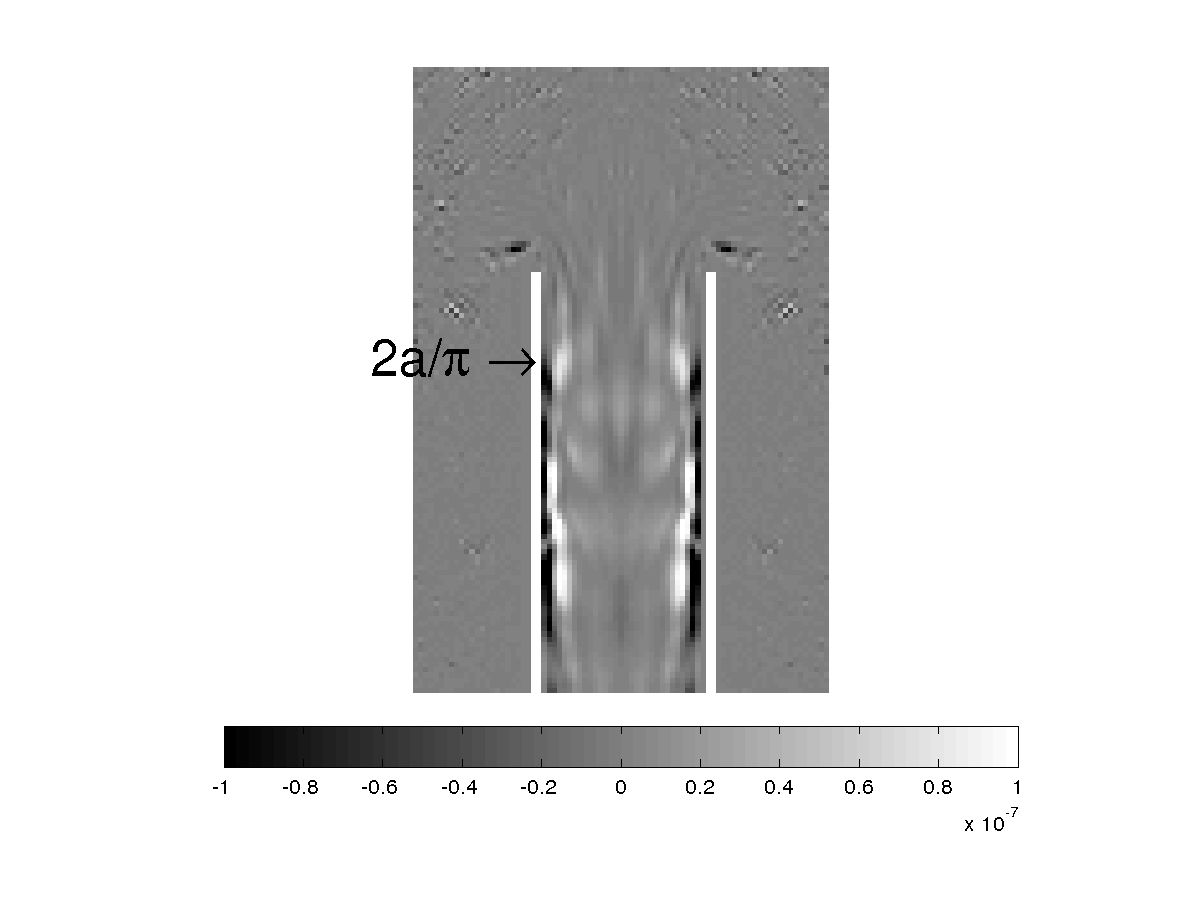
\includegraphics[width=1.1\linewidth]{figuras/max_007_media.png}
  \caption{$St = \pi/2$}
  \label{fig:comparacao_007_max}
\end{subfigure}%
\begin{subfigure}{0.5\textwidth}
  \centering
  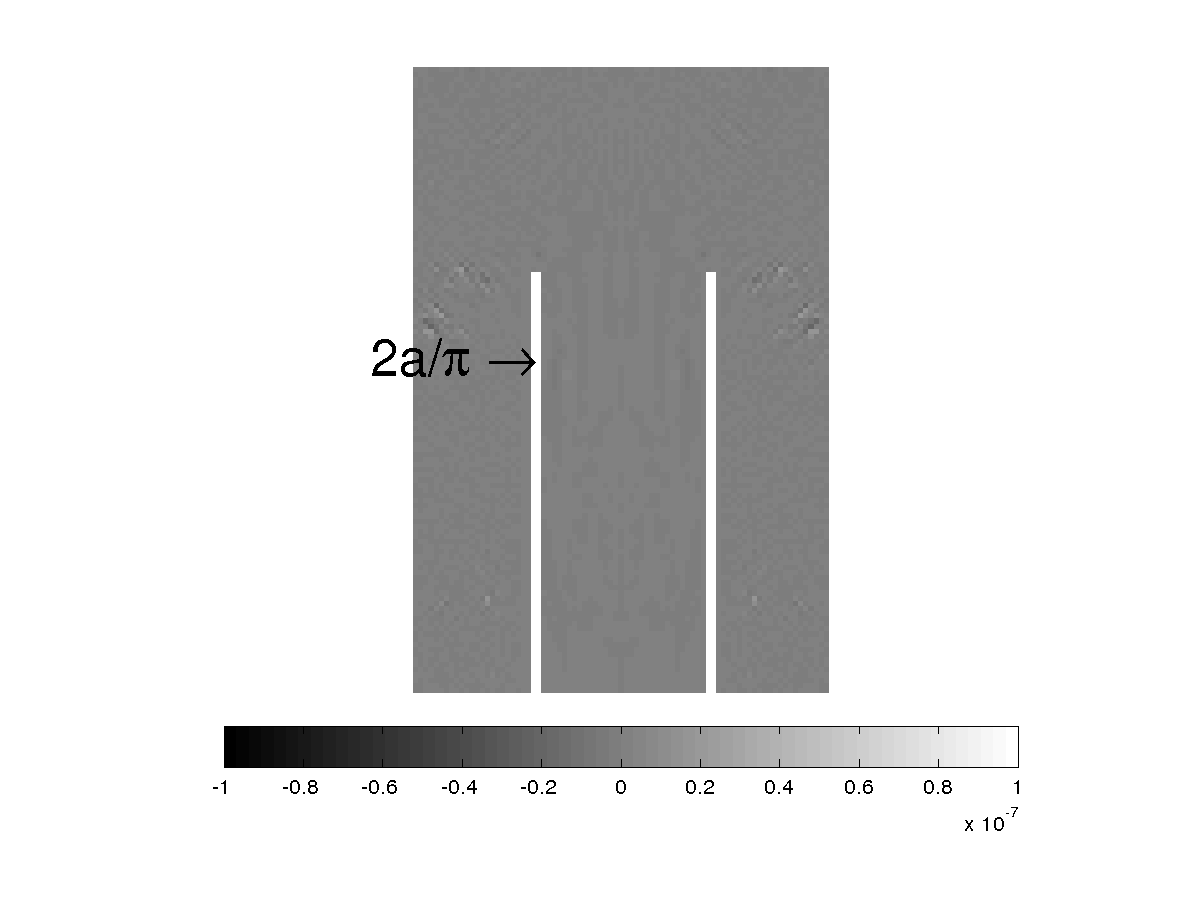
\includegraphics[width=1.1\linewidth]{figuras/min_007_media.png}
  \caption{$St = 6,8$}
  \label{fig:comparacao_007_min}
\end{subfigure}
\caption[Comparação da média da potência acústica por unidade de volume ao longo de um período de oscilação para $M = 0,07$ e números de Strouhal $St = \pi/2$ e $St = 6,8$.]{Comparação da média da potência acústica por unidade de volume ao longo de um período de oscilação para $M = 0,07$ e números de Strouhal $St = \pi/2$ (\ref{fig:comparacao_007_max}) e $St = 6,8$ (\ref{fig:comparacao_007_min}).}
\label{fig:comparacao_007_media}
\end{figure}

\newpage
Também pode-se calcular a média da potência acústica por unidade de volume ao longo de um período de oscilação através da Equação (\ref{eq:integral_howe_2}). A Figura \ref{fig:comparacao_007_media} apresenta os resultados desse cálculo para $M = 0,07$ e números de Strouhal $St = \pi/2$ e $St = 6,8$. As regiões tendendo para o branco e as regiões tendendo para o preto equivalem a regiões de geração e absorção de energia acústica respectivamente. É possível observar na Figura \ref{fig:comparacao_007_max} a geração de energia acústica na região de $2a/\pi$, como também outras regiões com geração e absorção de energia acústica não relacionadas ao fenômento abordado de desprendimento de vórtices. Quanto a Figura \ref{fig:comparacao_007_min} observa-se um comportamento homogêneo ao longo de toda região de análise.    

Novamente, com o uso da Equação (\ref{eq:integral_howe_2}), é possível calcular a potência acústica instantânea por unidade de volume em cada instante de tempo num mapa de valores, referenciando regiões de geração e absorção de energia acústica como áreas tendendo para o branco e o preto respectivamente. A Figura \ref{fig:max_007} apresenta  esse cálculo para $M = 0,07$ e $St = \pi/2$. É visível zonas de geração e absorção de energia acústica ao longo de cada instante. Já a Figura \ref{fig:min_007} apresenta a energia acústica instantânea para $M = 0,07$ e $St = 6,8$ e, como nessa frequência não há o desenvolvimento do fenômeno abordado, há a ausência de regiões de geração e absorção de energia acústica, principalmente nas regiões citadas anteriormente.

\begin{landscape}
\newpage
\vfill
\begin{figure}[ht!]
\begin{subfigure}{0.55 \textwidth}
  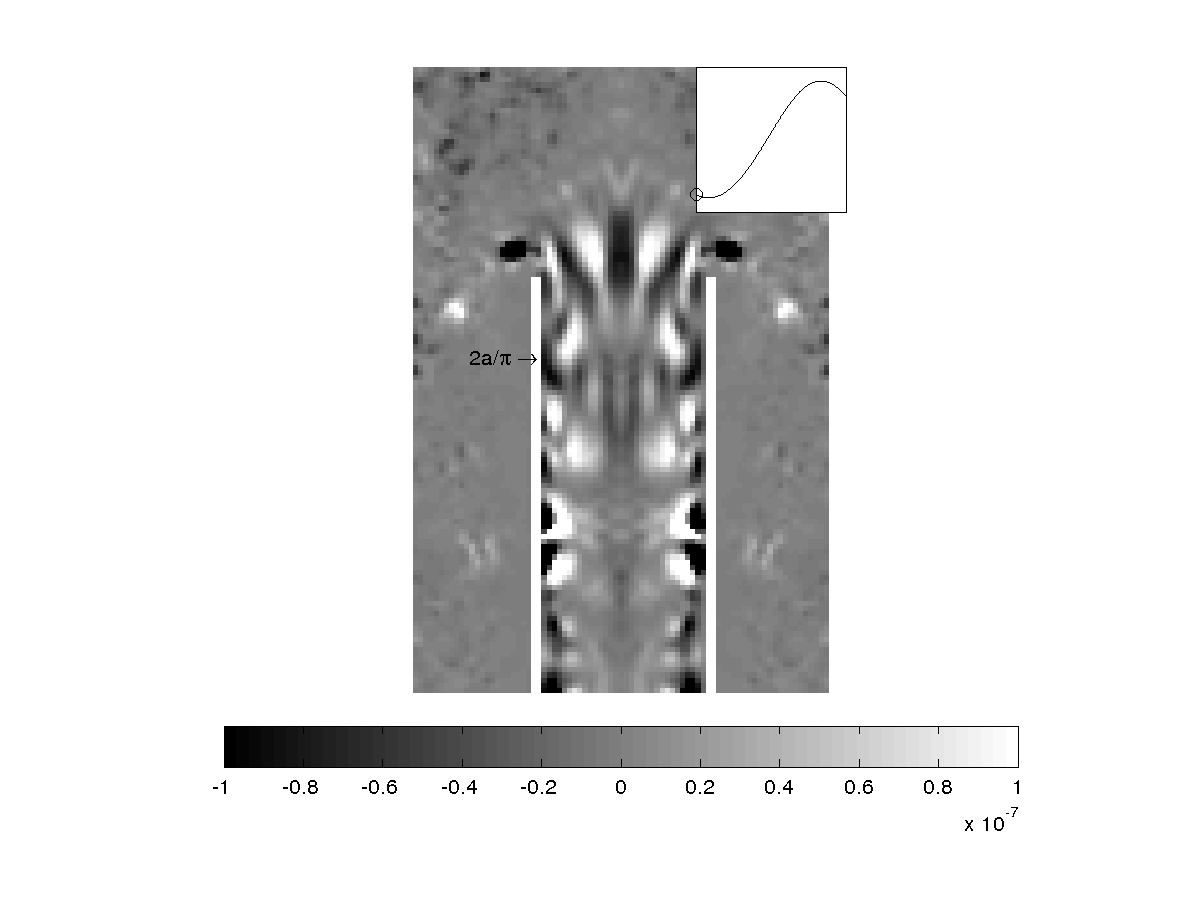
\includegraphics[width=1.\linewidth]{figuras/max_ka_007_1.png}
  \caption[]{}
  \label{fig:max_007_1}
\end{subfigure}
\begin{subfigure}{0.55 \textwidth}
  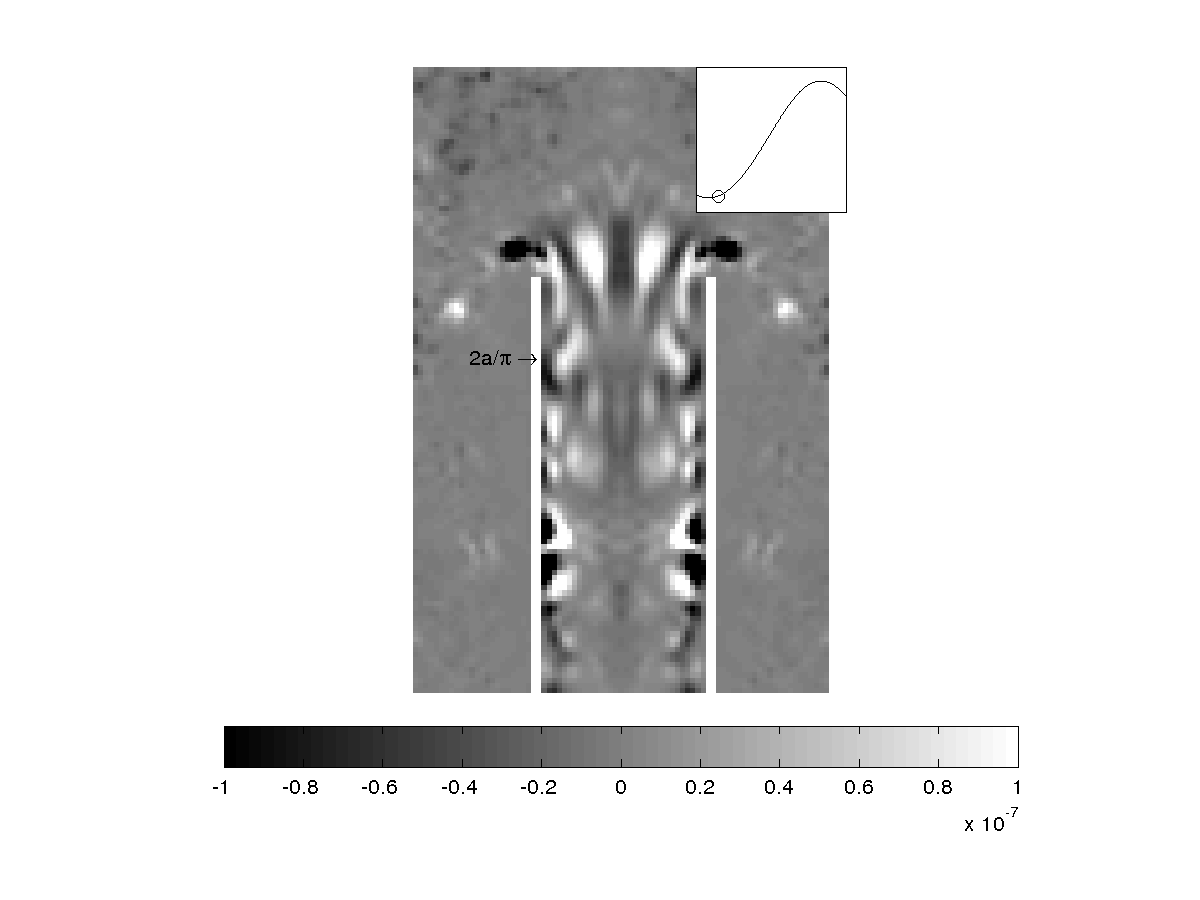
\includegraphics[width=1.\linewidth]{figuras/max_ka_007_2.png}
  \caption[]{}
  \label{fig:max_007_2}
\end{subfigure}
\begin{subfigure}{0.55 \textwidth}
  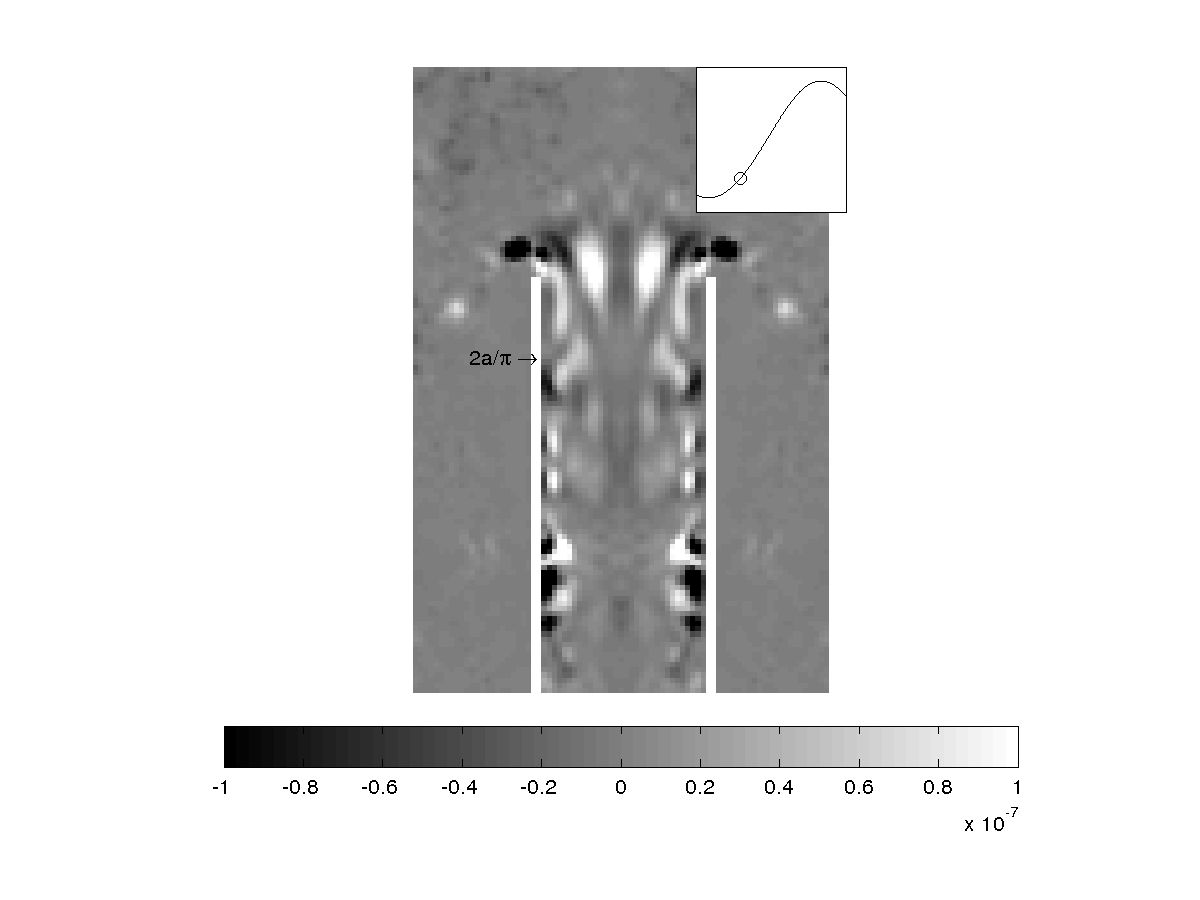
\includegraphics[width=1.\linewidth]{figuras/max_ka_007_3.png}
  \caption[]{}
  \label{fig:max_007_3}
\end{subfigure}
\par\medskip
\begin{subfigure}{0.55 \textwidth}
  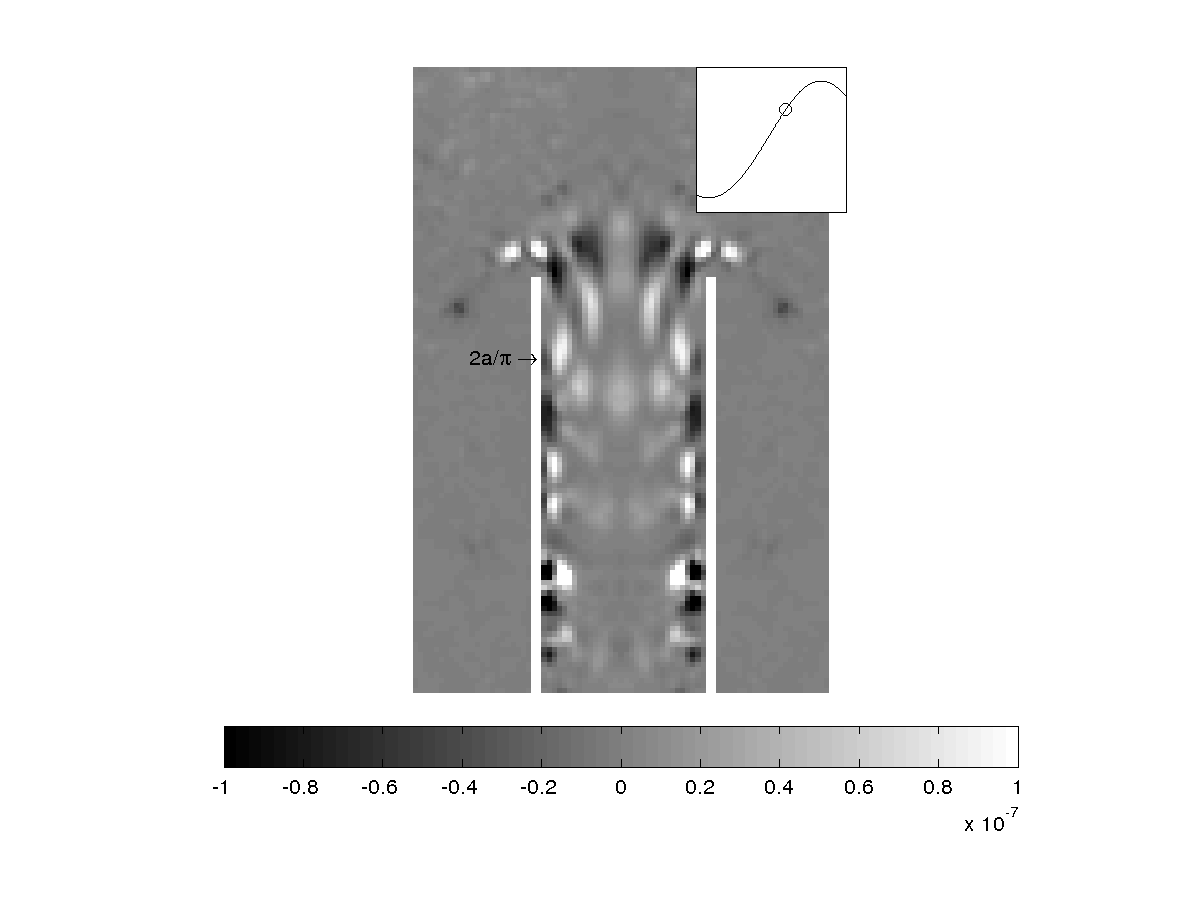
\includegraphics[width=1.\linewidth]{figuras/max_ka_007_4.png}
  \caption[]{}
  \label{fig:max_007_4}
\end{subfigure}
\begin{subfigure}{0.55 \textwidth}
  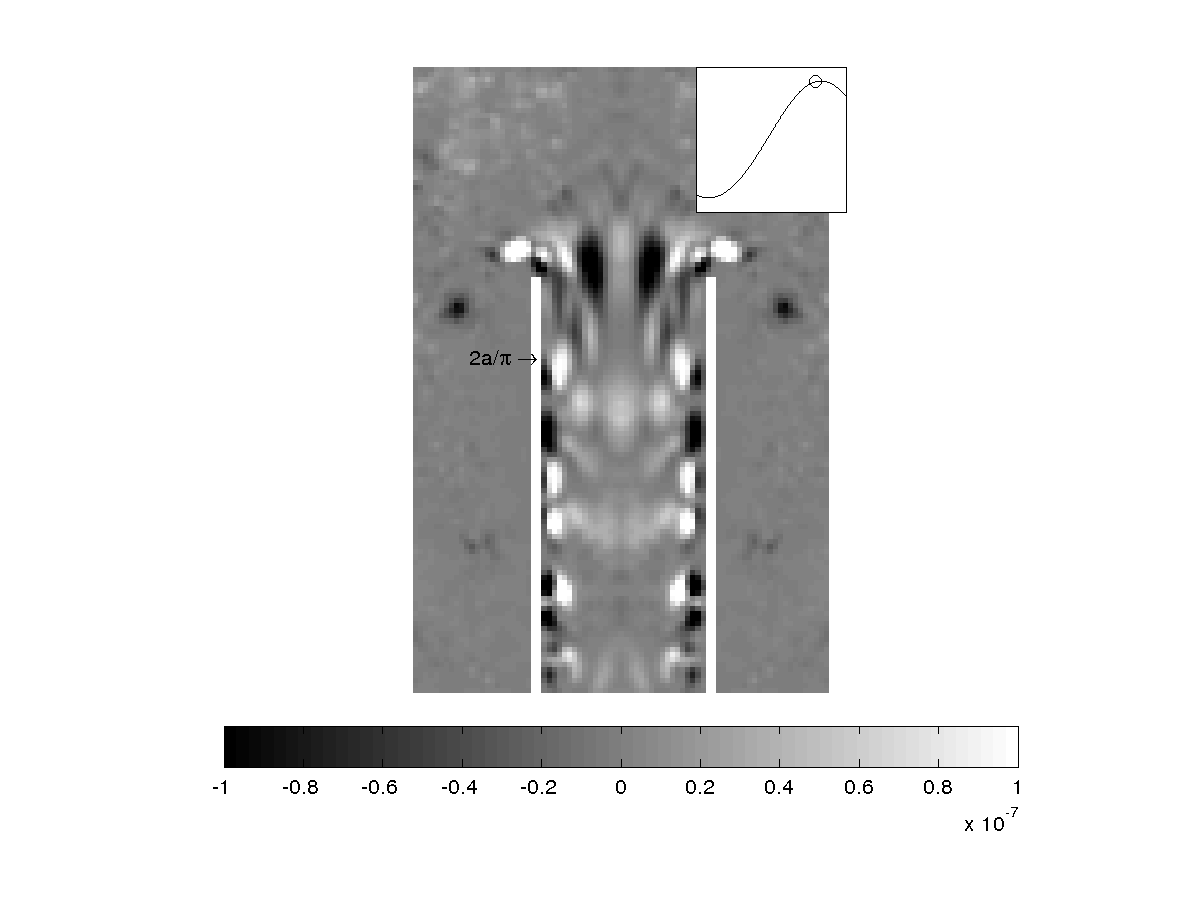
\includegraphics[width=1.\linewidth]{figuras/max_ka_007_5.png}
  \caption[]{}
  \label{fig:max_007_5}
\end{subfigure}
\begin{subfigure}{0.55 \textwidth}
  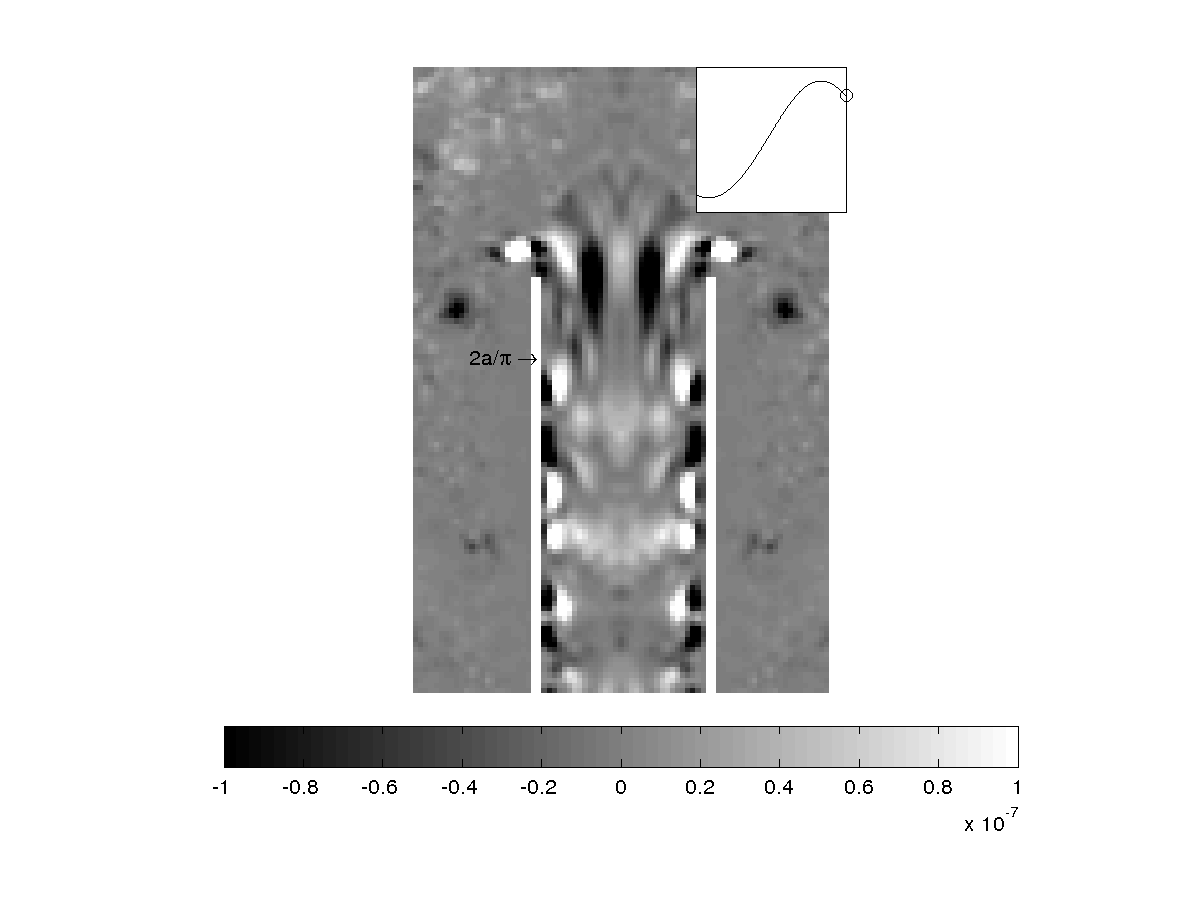
\includegraphics[width=1.\linewidth]{figuras/max_ka_007_6.png}
  \caption[]{}
  \label{fig:max_007_6}
\end{subfigure}
\caption[Potência acústica instantânea por unidade de volume para $M = 0,07$ e $St = \pi/2$.]{Potência acústica instantânea por unidade de volume no interior do duto para $M = 0,07$ e $St = \pi/2$.}\label{fig:max_007}
\end{figure}
\vfill
\clearpage
\end{landscape}


\begin{landscape}
\newpage
\vfill
\begin{figure}[ht!]
\begin{subfigure}{0.55 \textwidth}
  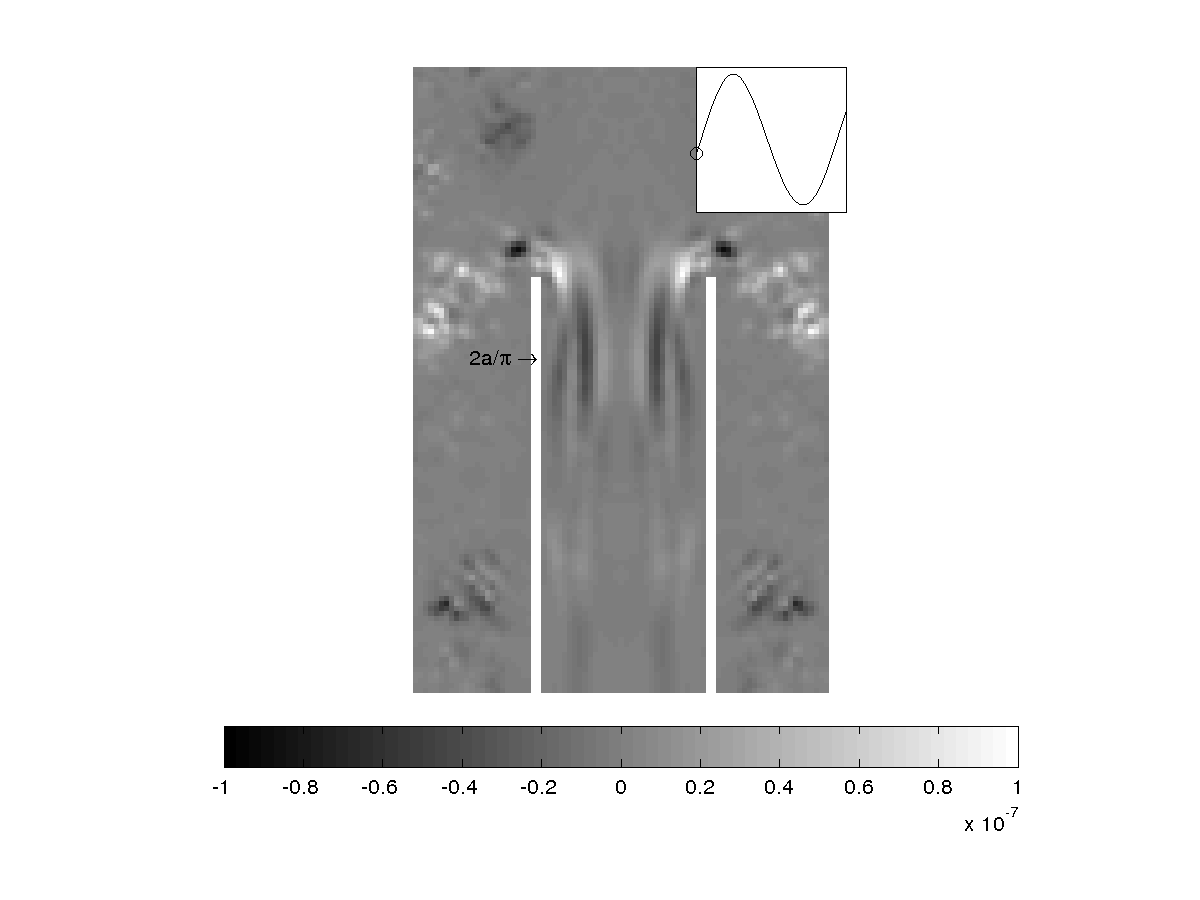
\includegraphics[width=1.\linewidth]{figuras/min_ka_007_1.png}
  \caption[]{}
  \label{fig:min_007_1}
\end{subfigure}
\begin{subfigure}{0.55 \textwidth}
  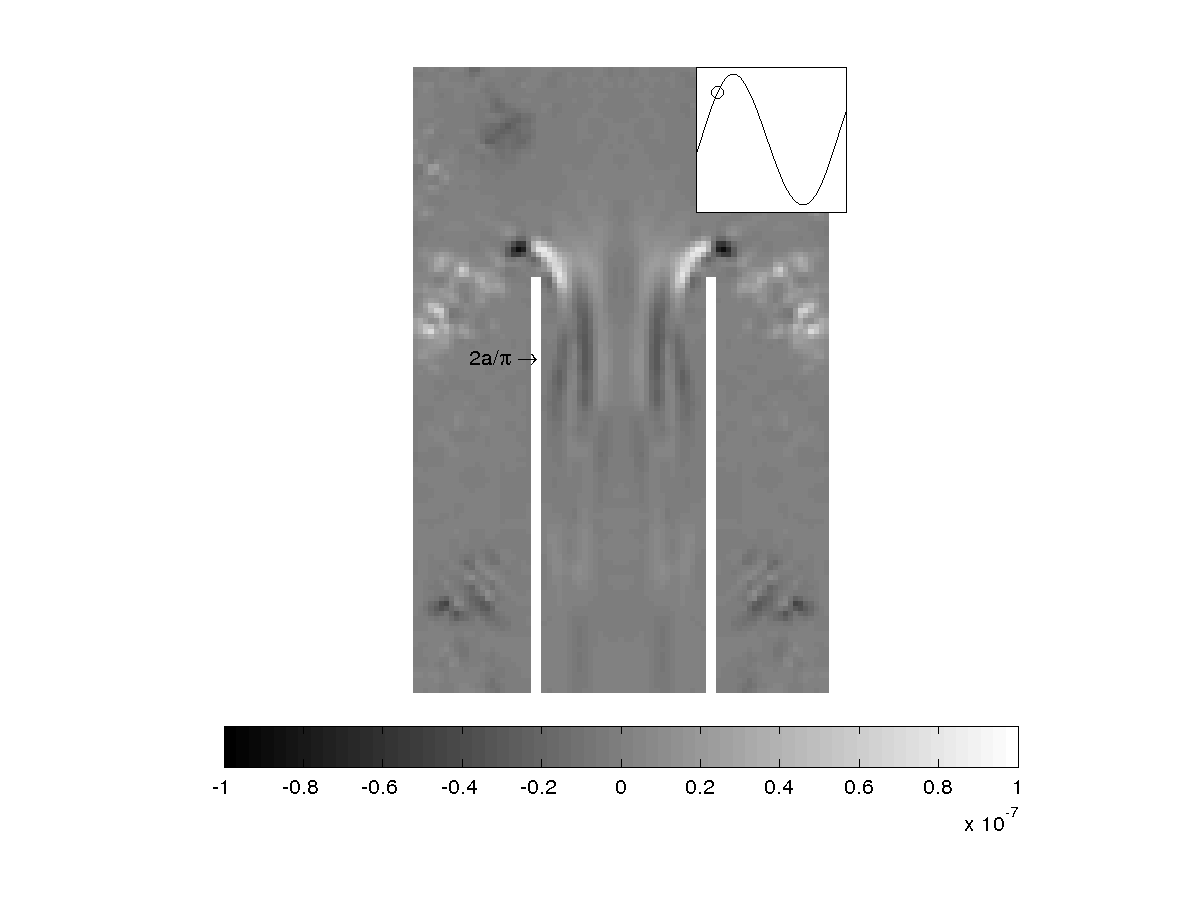
\includegraphics[width=1.\linewidth]{figuras/min_ka_007_2.png}
  \caption[]{}
  \label{fig:min_007_2}
\end{subfigure}
\begin{subfigure}{0.55 \textwidth}
  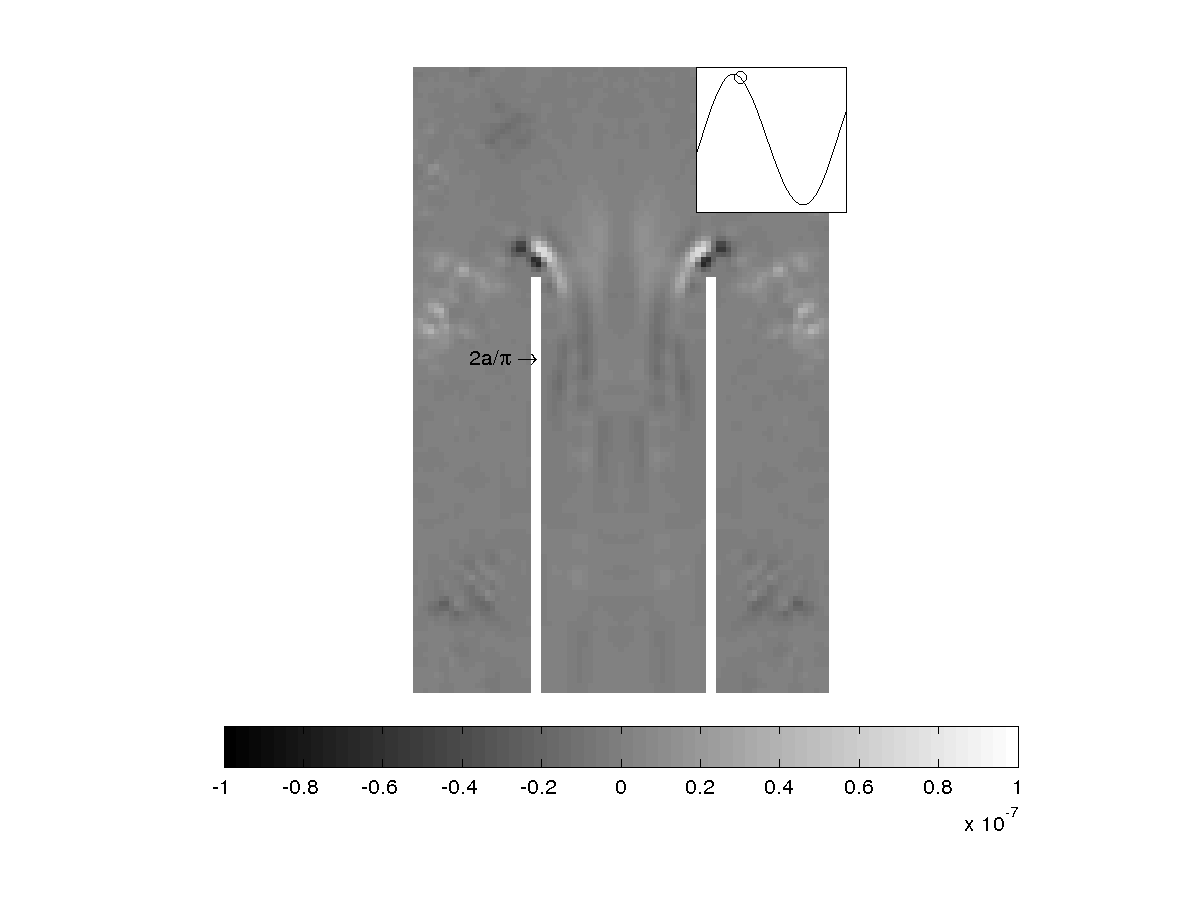
\includegraphics[width=1.\linewidth]{figuras/min_ka_007_3.png}
  \caption[]{}
  \label{fig:min_007_3}
\end{subfigure}
\par\medskip
\begin{subfigure}{0.55 \textwidth}
  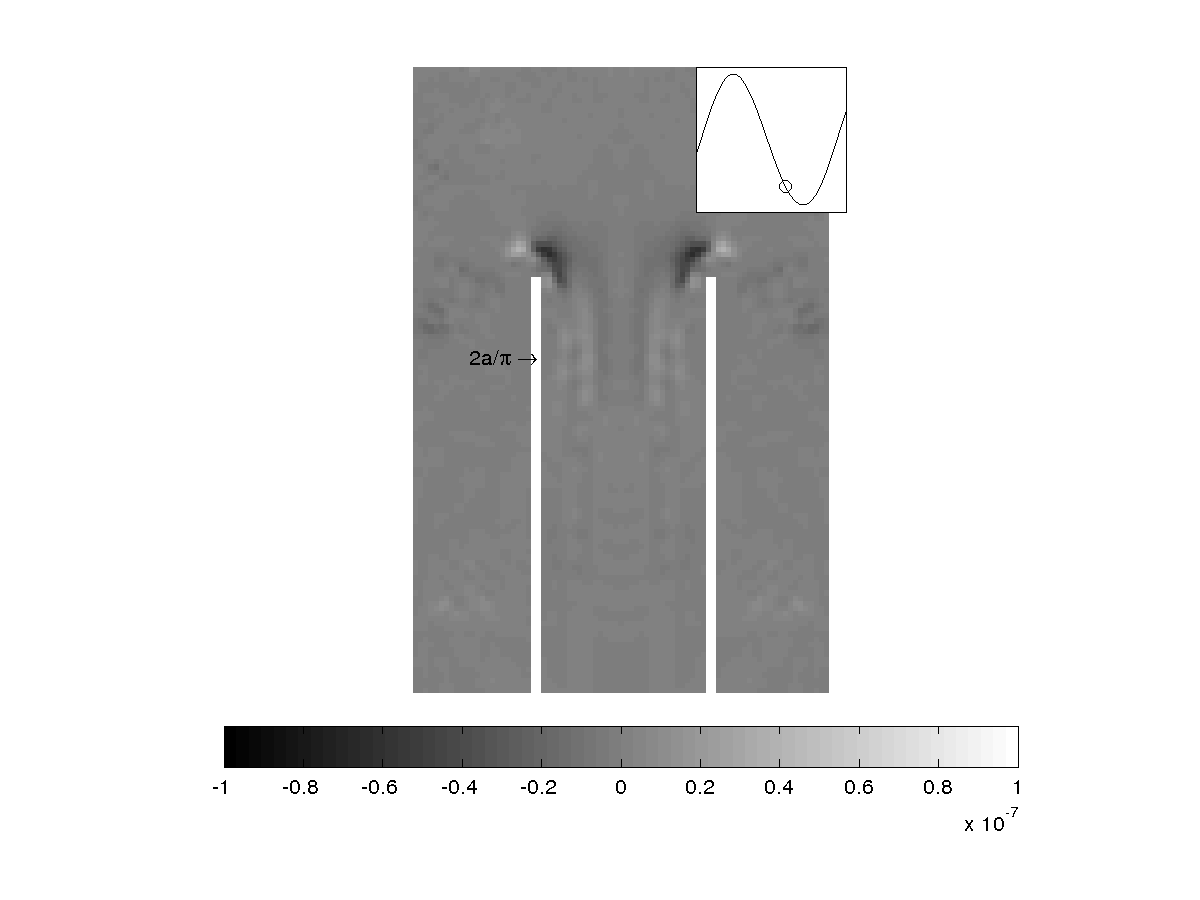
\includegraphics[width=1.\linewidth]{figuras/min_ka_007_4.png}
  \caption[]{}
  \label{fig:min_007_4}
\end{subfigure}
\begin{subfigure}{0.55 \textwidth}
  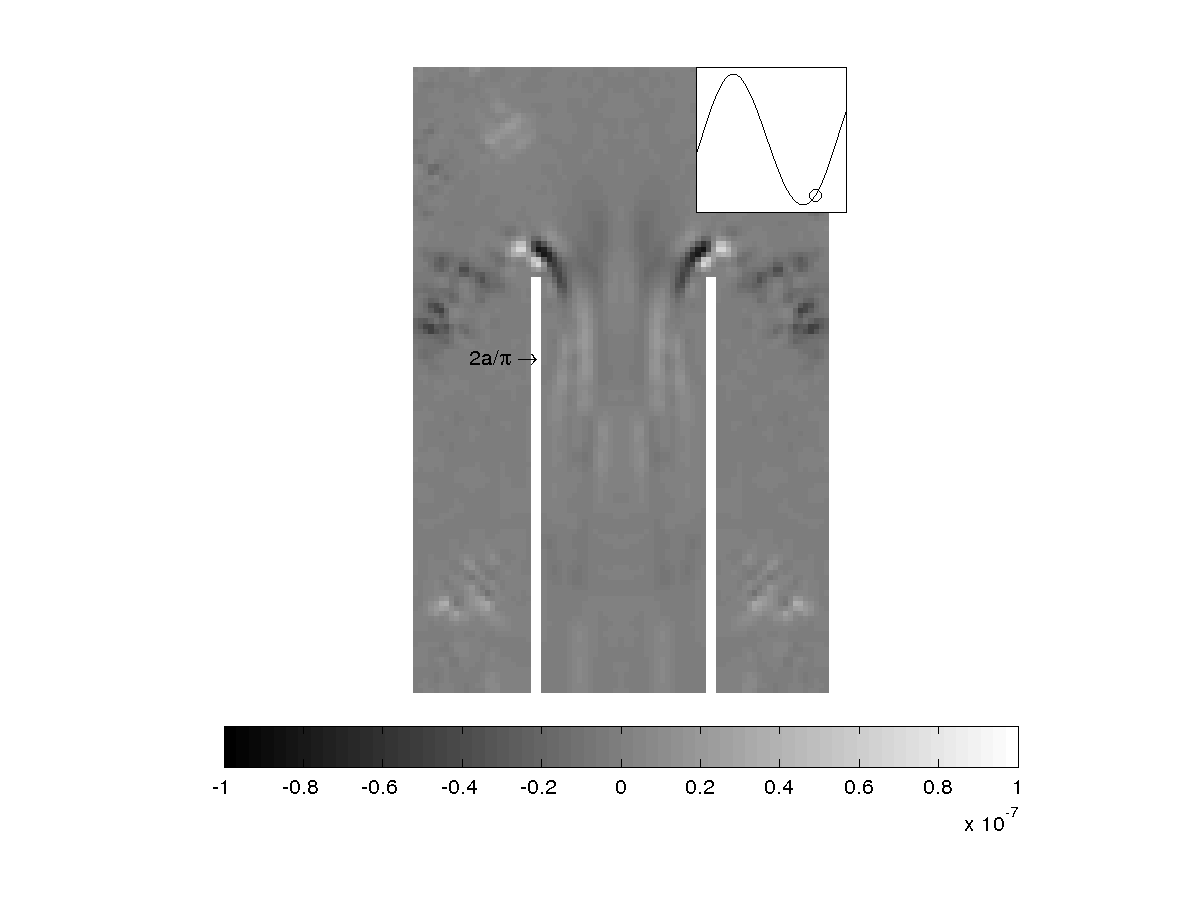
\includegraphics[width=1.\linewidth]{figuras/min_ka_007_5.png}
  \caption[]{}
  \label{fig:min_007_5}
\end{subfigure}
\begin{subfigure}{0.55 \textwidth}
  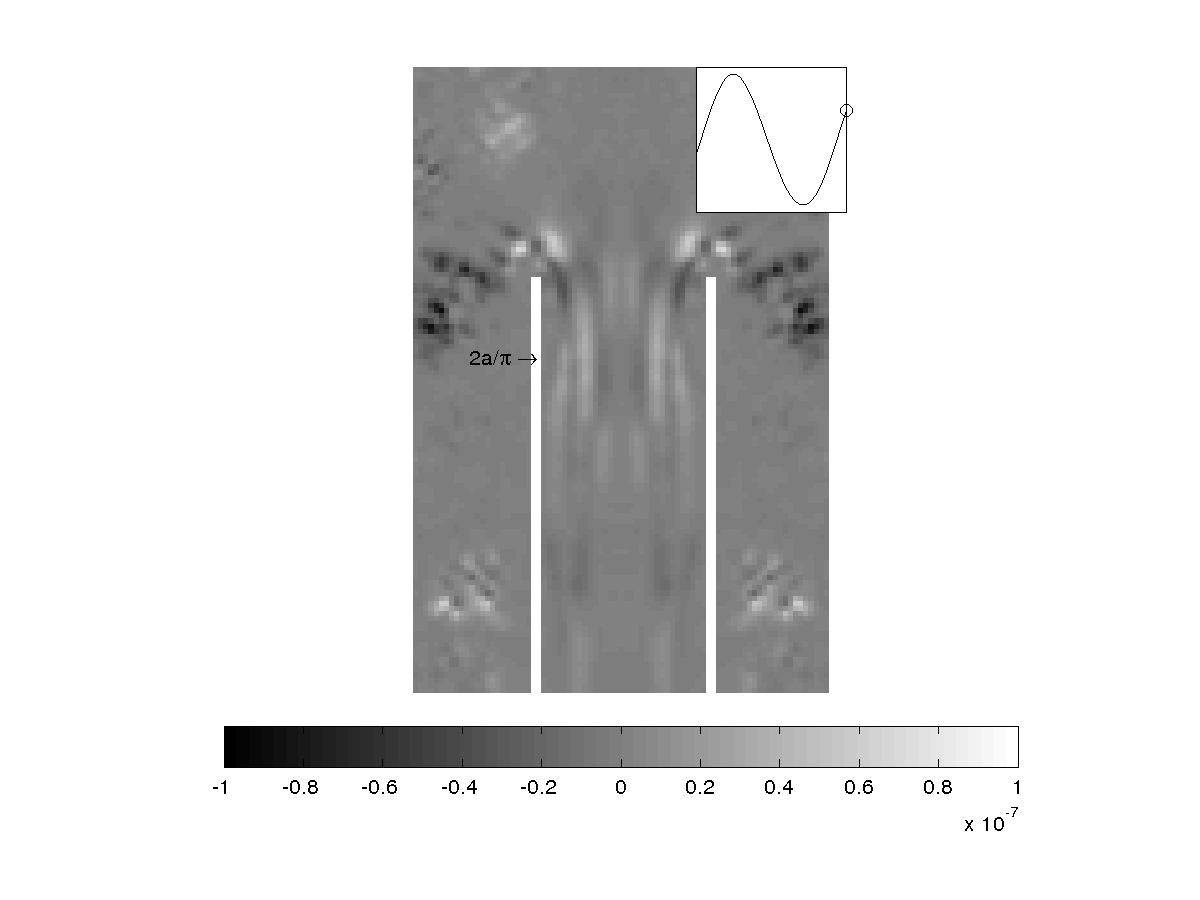
\includegraphics[width=1.\linewidth]{figuras/min_ka_007_6.png}
  \caption[]{}
  \label{fig:min_007_6}
\end{subfigure}
\caption[Potência acústica instantânea por unidade de volume para $M = 0,07$ e $St = 6,8$.]{Potência acústica instantânea por unidade de volume no interior do duto para $M = 0,07$ e $St = 6,8$.}\label{fig:min_007}
\end{figure}
\vfill
\clearpage
\end{landscape}

Em vista do que foi exposto e concernente a primeira pergunta, o fenômeno da amplificação de $|R_{e}|$ para $M = 0,07$ e $St \sim \pi/2$, constatado na Figura \ref{fig:abs_r_sugado_strouhal_energy}, ocorre devido ao surgimento de zonas de geração de energia acústica dentro do duto próximas a região $2a/\pi$. Tal fenômeno não ocorre quando $St \neq \pi/2$. Esse fato corrobora com a hipótese de que a energia vorticial do fluido é convertida em energia acústica nesse contexto.

Com relação a segunda pergunta, pode-se investigar o efeito de $|R_{r}|$ fixado em $St \sim \pi/2$ com relação aos números de Mach através da integral de energia de Howe apresentada na Equação (\ref{eq:integral_howe_1}). Em vista disso, a potência acústica média gerada ao longo de um período para $M = 0,07$ e $M = 0,1$, calculada na região entre a terminação e $2a/\pi$ para o interior do duto, é apresentada na Tabela \ref{table:potencia_mach}. Pode-se perceber que o fenômeno da amplificação é atenuado quando o número de Mach é maior que $0,07$. 

\begin{table}[ht!]
\centering
\caption{Potência acústica calculada ao longo de um período de onda para $St = \pi/2$ e diferentes números de Mach.}
\label{table:potencia_mach}
    \begin{tabular}{|l|l|l|l|}
        \hline
        $M$ & $<P>$ \\ \hline
        $0,07$ & 4,6173e-06  \\ \hline  
        $0,1$ & 6,1312e-07 \\ \hline
    \end{tabular}
\end{table}

\begin{figure}[ht!]
\begin{subfigure}{0.5\textwidth}
  \centering
  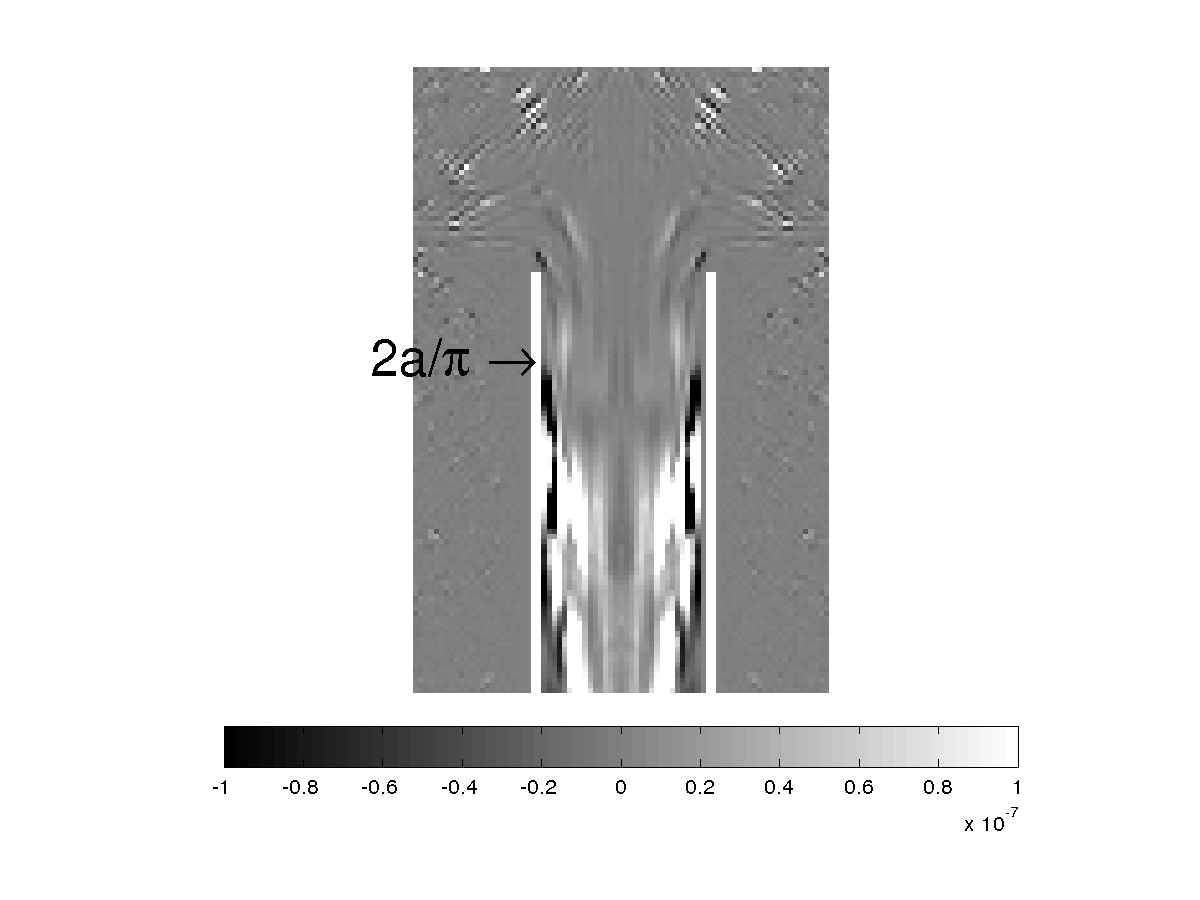
\includegraphics[width=1.1\linewidth]{figuras/max_01_media.png}
  \caption{$M = 0,1$}
  \label{fig:comparacao_01}
\end{subfigure}%
\begin{subfigure}{0.5\textwidth}
  \centering
  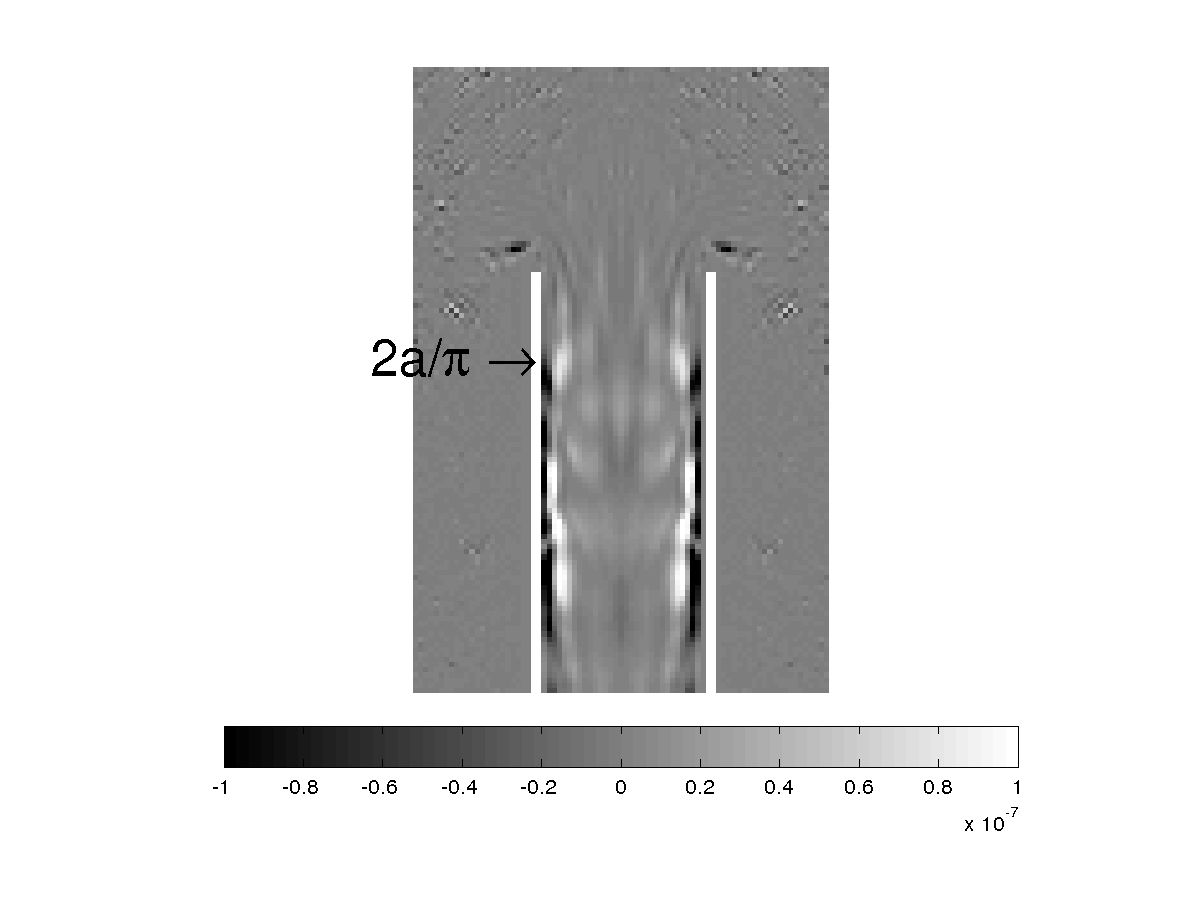
\includegraphics[width=1.1\linewidth]{figuras/max_007_media.png}
  \caption{$M = 0,07$}
  \label{fig:comparacao_007}
\end{subfigure}
\caption[Comparação da média da potência acústica por unidade de volume ao longo de um período entre $M = 0,1$ e $M = 0,07$ para $St = \pi/2.$]{Comparação da média da potência acústica por unidade de volume ao longo de um período entre $M = 0,1$ (\ref{fig:comparacao_01}) e $M = 0,07$ (\ref{fig:comparacao_007}) para $St = \pi/2.$}
\label{fig:comparacao_007_01}
\end{figure}

\newpage
Usando a Equação (\ref{eq:integral_howe_2}), pode-se obter a média da potência acústica por unidade de volume ao longo de um período de oscilação. A Figura \ref{fig:comparacao_007_01} mostra a comparação desse parâmetro em mapas de valores, sendo zonas de geração e absorção de energia acústica as regiões brancas e pretas respectivamente. Pode-se observar que \ref{fig:comparacao_01} possui uma energia menor na região de $2a/\pi$ de distância, ou seja, há mais energia acústica sendo gerada para $M = 0,07$ do que $M = 0,1$. Pode-se observar também que, para outras regiões do duto, \ref{fig:comparacao_01} possui mais zonas de geração de energia acústica do que \ref{fig:comparacao_007}, entretanto subentende-se que esse fenômeno não está relacionado diretamente com a fenomenologia abordada nos resultados da Figura \ref{fig:abs_r_sugado_strouhal_mach}.   

Pode-se também, com o uso da Equação (\ref{eq:integral_howe_2}), calcular a potência acústica instantânea por unidade de volume em cada instante de tempo num mapa de valores, referenciando regiões tendendo para o branco e para o preto como zonas de geração e absorção de energia acústica respectivamente. A Figura \ref{fig:max_01} apresenta esse cálculo para $M = 0,10$ e $St = \pi/2$ e é possível observar zonas de geração e absorção de energia acústica ao longo de cada instante. Vale ressaltar que nas Figuras \ref{fig:max_01_5} e \ref{fig:max_01_6} apresentam um fenômeno que é ausente nos resultados da Figura \ref{fig:max_007} para $M = 0,07$: o surgimento de uma zona de absorção acústica na região de $2a/\pi$ de distância em relação a terminação. Tal fato ocasiona uma redução significativa na média da potência acústica apresentada na Tabela \ref{table:potencia_mach}, eclodindo no comportamento de declínio e não monotonocidade da Figura \ref{fig:abs_r_sugado_strouhal_mach}.

Em vista do que foi apresentado e concernente a segunda pergunta, infere-se que o valor máximo de $|R_{r}|$ para $St \sim \pi/2$, constatado na Figura \ref{fig:abs_r_sugado_strouhal_mach}, ocorre devido ao surgimento de zonas de absorção de energia acústica dentro do duto próximas a região $2a/\pi$, apresentadas nas Figuras \ref{fig:max_01_5} e \ref{fig:max_01_6}. Tal fenômeno ocorre a partir do número de $M = 0,10$ e subentende-se que se intensifica a medida que o número Mach aumenta, ocasionando no declínio do módulo do coeficiente reflexão na terminação quando $St = \pi/2$.

\begin{landscape}
\newpage
\vfill
\begin{figure}[ht!]
\begin{subfigure}{0.55 \textwidth}
  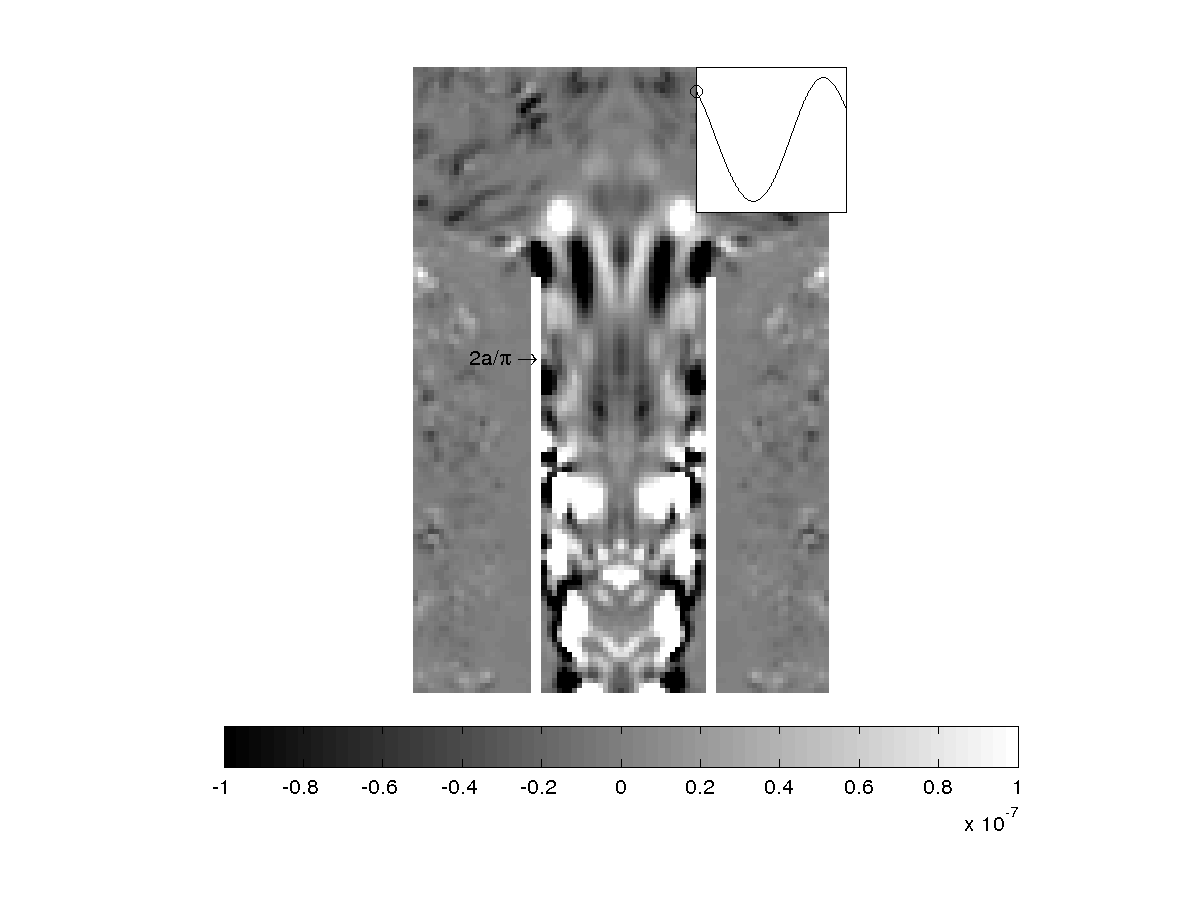
\includegraphics[width=1.\linewidth]{figuras/max_ka_01_1.png}
  \caption[]{}
  \label{fig:max_01_1}
\end{subfigure}
\begin{subfigure}{0.55 \textwidth}
  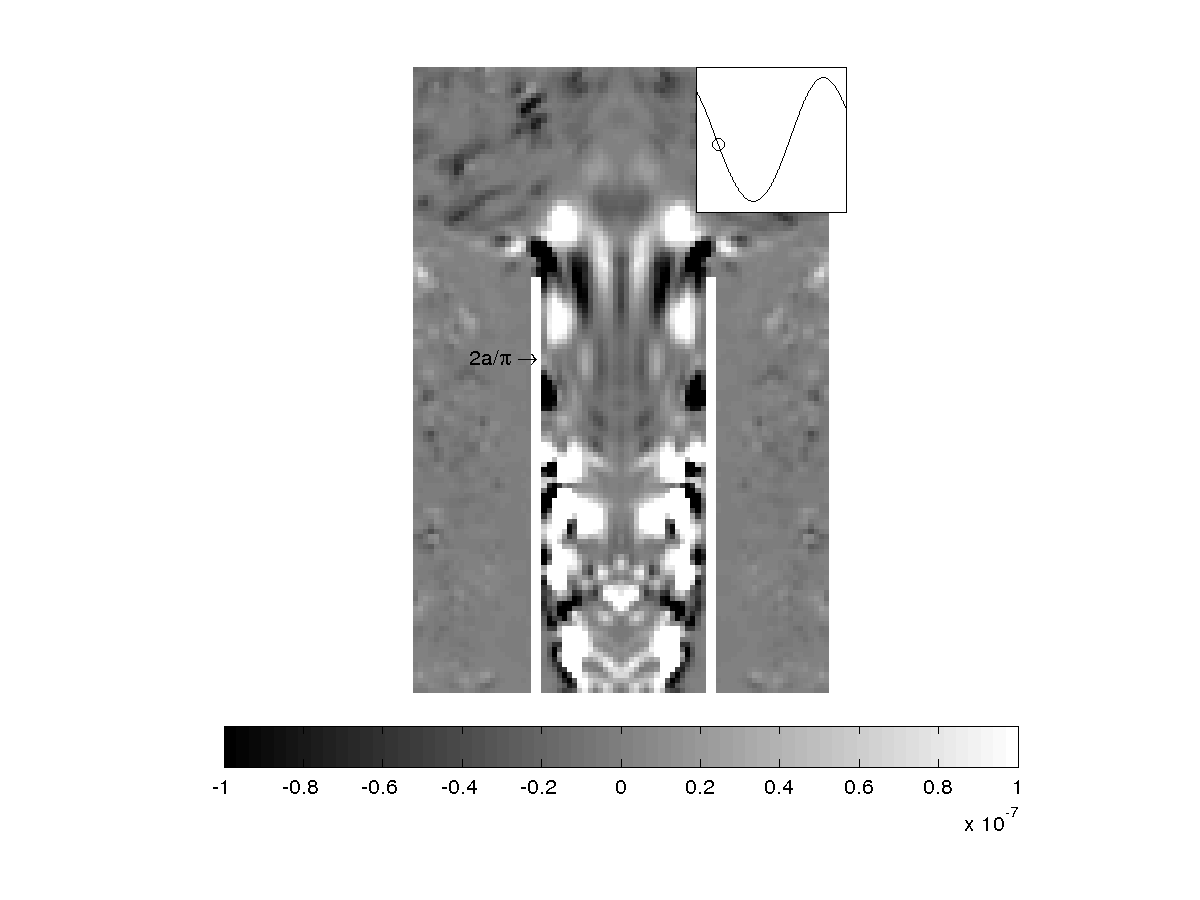
\includegraphics[width=1.\linewidth]{figuras/max_ka_01_2.png}
  \caption[]{}
  \label{fig:max_01_2}
\end{subfigure}
\begin{subfigure}{0.55 \textwidth}
  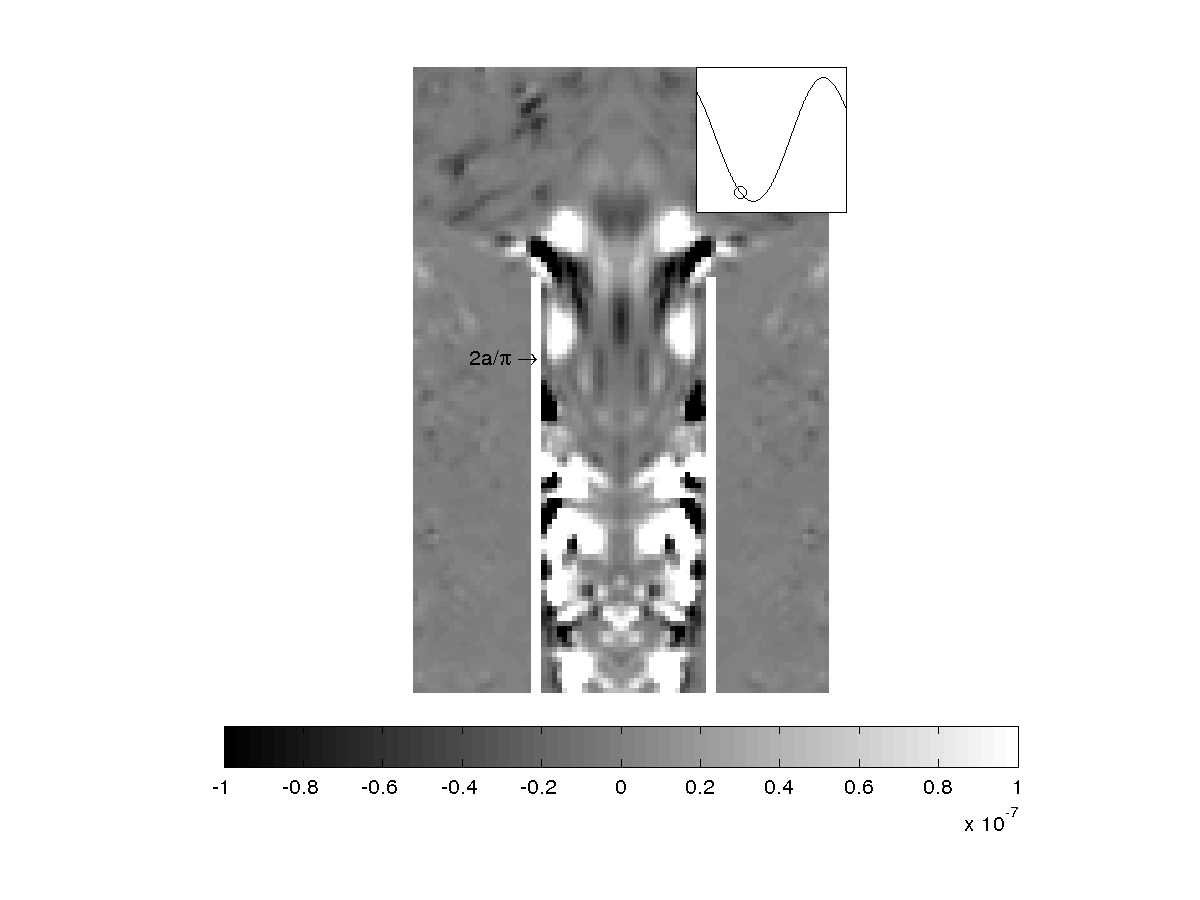
\includegraphics[width=1.\linewidth]{figuras/max_ka_01_3.png}
  \caption[]{}
  \label{fig:max_01_3}
\end{subfigure}
\par\medskip
\begin{subfigure}{0.55 \textwidth}
  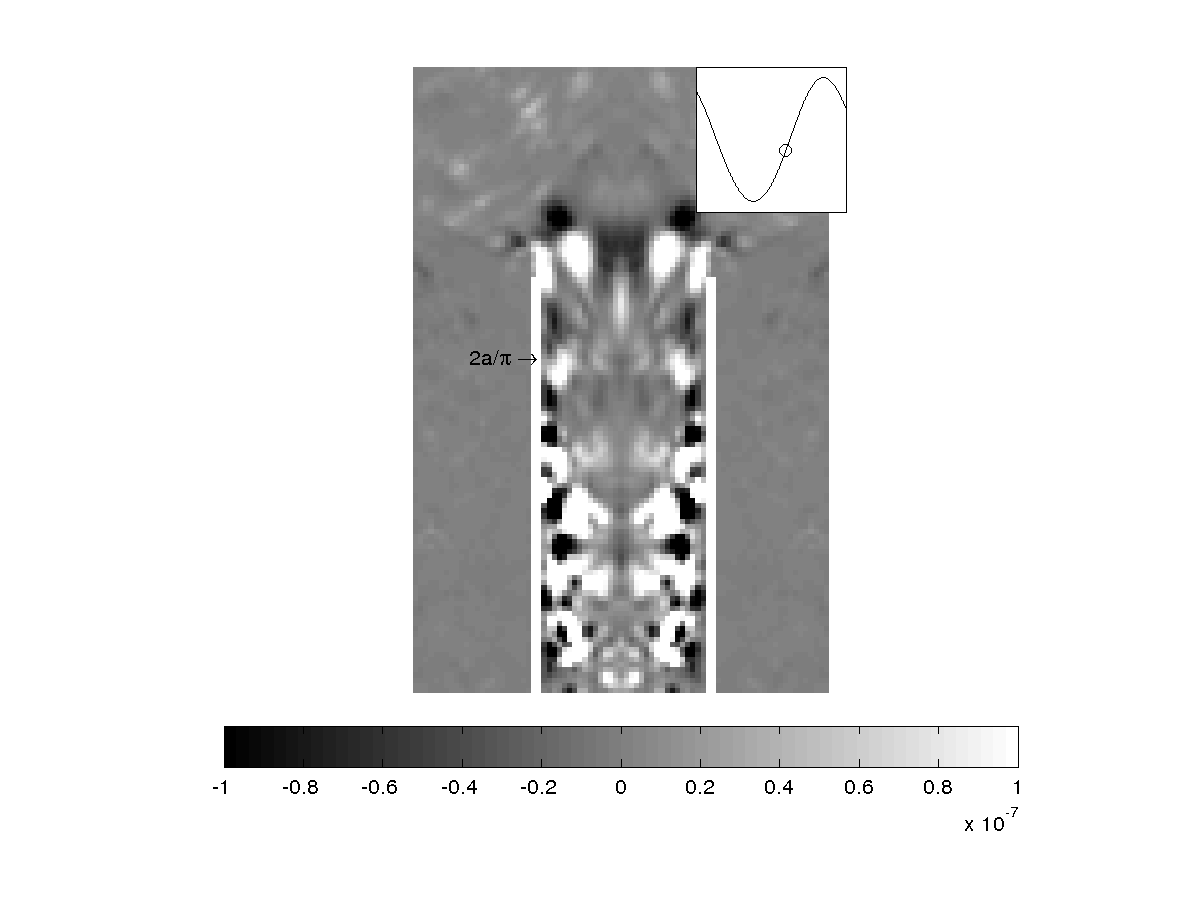
\includegraphics[width=1.\linewidth]{figuras/max_ka_01_4.png}
  \caption[]{}
  \label{fig:max_01_4}
\end{subfigure}
\begin{subfigure}{0.55 \textwidth}
  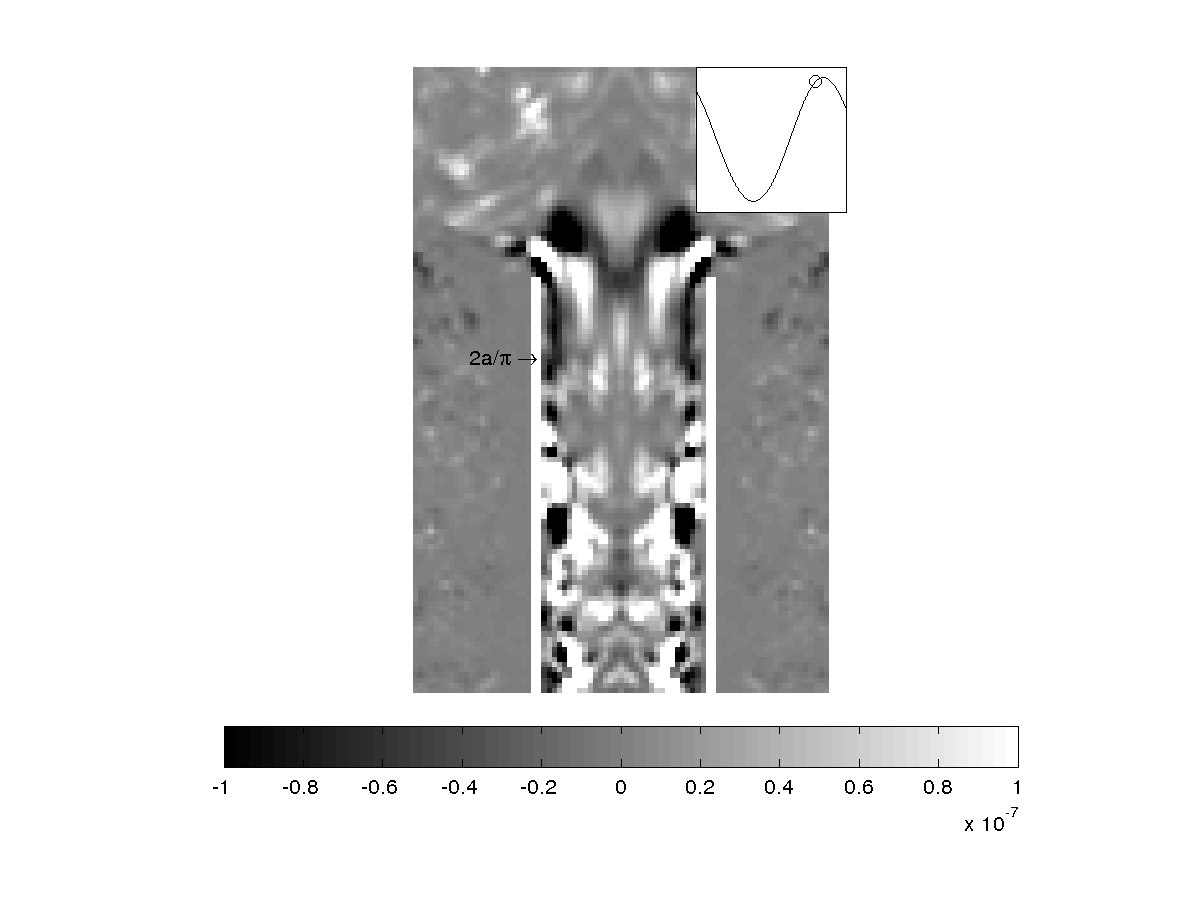
\includegraphics[width=1.\linewidth]{figuras/max_ka_01_5.png}
  \caption[]{}
  \label{fig:max_01_5}
\end{subfigure}
\begin{subfigure}{0.55 \textwidth}
  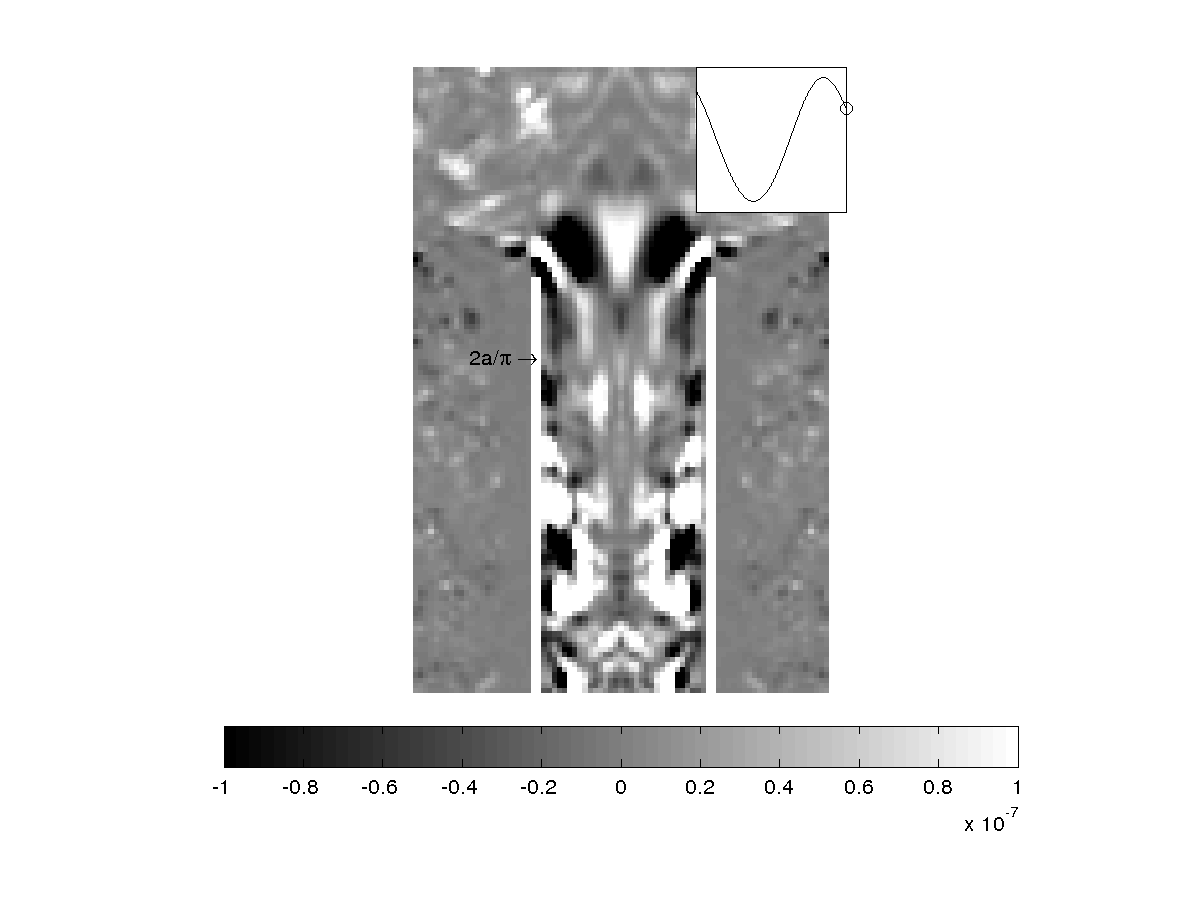
\includegraphics[width=1.\linewidth]{figuras/max_ka_01_6.png}
  \caption[]{}
  \label{fig:max_01_6}
\end{subfigure}
\caption[Energia acústica para $M = 0,07$ e $St = \pi/2$.]{Energia acústica no interior do duto para $M = 0,1$ e $St = \pi/2$.}\label{fig:max_01}
\end{figure}
\vfill
\clearpage
\end{landscape}

%\newpage
%\begin{figure}[ht!]
%\centering
  %\begin{tikzpicture}
  \begin{axis}[
  width=0.9\textwidth,
  height=0.5\textwidth,
  x tick label style={
      /pgf/number format/.cd,
          fixed,
          fixed zerofill,
          precision=2,
      /tikz/.cd
  },
  xmin=0.05,
  xmax=0.2,
  ymin=0.,
  ymax=0.7,
  ytick distance=0.1,
  xtick distance=0.03,
  grid=major, % Display a grid  
  %grid style={dashed,gray!90}, % Set the style
  xlabel = $M$,
  ylabel = $l/a$,
  ]
 \addplot[color=black, thick] table[x index=0,y index=1] {dados/duto_sugado/loa_strouhal_mach.txt};

  \end{axis}
  \end{tikzpicture}
  \caption[Coeficiente de correção da terminação $l/a$ com escoamento de exaustão em relação ao número de Mach ($M$) no Strouhal $St = \pi/2$]{Resultado de coeficientes de correção da terminação $l/a$ fixados no Strouhal $St = \pi/2$ em relação ao número de Mach ($M$) para escoamentos sugados. Os resultados foram calculados no ponto $\textbf{P}$ na terminação do duto.}

  \label{fig:loa_sugado_strouhal_mach}
%\end{figure}

%valores de perda de carga:
%0.05 = 0.49
%0.07 = 0.59
%0.1 = 0.71
%0.15 = 0.74
%0.2 = 0.75
